\documentclass[a4paper,12pt,twoside]{article}\usepackage[]{graphicx}\usepackage[]{color}
%% maxwidth is the original width if it is less than linewidth
%% otherwise use linewidth (to make sure the graphics do not exceed the margin)
\makeatletter
\def\maxwidth{ %
  \ifdim\Gin@nat@width>\linewidth
    \linewidth
  \else
    \Gin@nat@width
  \fi
}
\makeatother

\definecolor{fgcolor}{rgb}{0.345, 0.345, 0.345}
\newcommand{\hlnum}[1]{\textcolor[rgb]{0.686,0.059,0.569}{#1}}%
\newcommand{\hlstr}[1]{\textcolor[rgb]{0.192,0.494,0.8}{#1}}%
\newcommand{\hlcom}[1]{\textcolor[rgb]{0.678,0.584,0.686}{\textit{#1}}}%
\newcommand{\hlopt}[1]{\textcolor[rgb]{0,0,0}{#1}}%
\newcommand{\hlstd}[1]{\textcolor[rgb]{0.345,0.345,0.345}{#1}}%
\newcommand{\hlkwa}[1]{\textcolor[rgb]{0.161,0.373,0.58}{\textbf{#1}}}%
\newcommand{\hlkwb}[1]{\textcolor[rgb]{0.69,0.353,0.396}{#1}}%
\newcommand{\hlkwc}[1]{\textcolor[rgb]{0.333,0.667,0.333}{#1}}%
\newcommand{\hlkwd}[1]{\textcolor[rgb]{0.737,0.353,0.396}{\textbf{#1}}}%

\usepackage{framed}
\makeatletter
\newenvironment{kframe}{%
 \def\at@end@of@kframe{}%
 \ifinner\ifhmode%
  \def\at@end@of@kframe{\end{minipage}}%
  \begin{minipage}{\columnwidth}%
 \fi\fi%
 \def\FrameCommand##1{\hskip\@totalleftmargin \hskip-\fboxsep
 \colorbox{shadecolor}{##1}\hskip-\fboxsep
     % There is no \\@totalrightmargin, so:
     \hskip-\linewidth \hskip-\@totalleftmargin \hskip\columnwidth}%
 \MakeFramed {\advance\hsize-\width
   \@totalleftmargin\z@ \linewidth\hsize
   \@setminipage}}%
 {\par\unskip\endMakeFramed%
 \at@end@of@kframe}
\makeatother

\definecolor{shadecolor}{rgb}{.97, .97, .97}
\definecolor{messagecolor}{rgb}{0, 0, 0}
\definecolor{warningcolor}{rgb}{1, 0, 1}
\definecolor{errorcolor}{rgb}{1, 0, 0}
\newenvironment{knitrout}{}{} % an empty environment to be redefined in TeX

\usepackage{alltt}

% Gestion de la langue, des polices, ligatures, etc
\usepackage[utf8x]{inputenc}
\usepackage[english,francais]{babel}
\usepackage[babel]{microtype}

% Marges, interlignes, graphiques et colonnes multiples
\usepackage[top=2.5cm,bottom=2.5cm,left=3.5cm,right=2.5cm,twoside]{geometry}
\usepackage{setspace}
\usepackage{multicol}
\setlength\columnsep{10pt}
\usepackage{graphicx}
\onehalfspacing % interligne 1.5

% Gestion et mise en forme de la bibliographie
\usepackage[colon]{natbib}
\usepackage{breakcites}
\usepackage{spacecites}
% \addto{\captionsenglish}{\renewcommand{\bibname}{Références bibliographiques}}

% Création de 2 styles d'en-têtes et pieds de page : 1 pour le corps du texte et un pour la page de garde toc, etc
\usepackage{etoolbox,lastpage,fancyhdr}

\fancypagestyle{plain}{%
  \fancyhf{}%
  \fancyfoot{}%
  \renewcommand{\headrulewidth}{0pt}%
  \renewcommand{\footrulewidth}{0pt}%
}

\fancypagestyle{main}{%
  \fancyhead[L]{\emph{Université de La Rochelle}}
  \fancyhead[C]{}
  \fancyhead[R]{\emph{Master SPE}}
  \fancyfoot[L]{\emph{Pierre-Louis Stenger}}
  \fancyfoot[C]{}
  \fancyfoot[R]{\thepage\ / 43}
  \renewcommand{\headrulewidth}{0.4pt}
  \renewcommand{\footrulewidth}{0.4pt}
}

\appto\frontmatter{\pagestyle{plain}}
\appto\mainmatter{\pagestyle{main}}

% Quelques packages utiles (couleurs, liens dynamiques dans le pdf, gestion des unités, etc)
\usepackage[table,xcdraw]{xcolor}
\usepackage{frcursive}
\usepackage{nicefrac}
\usepackage[mediumspace,mediumqspace,Grey,squaren]{SIunits}
\usepackage[colorlinks,breaklinks,naturalnames,linkcolor=black,citecolor=black,menucolor=black,pagecolor=black,urlcolor=blue]{hyperref}  % ,backref=page
\usepackage{placeins}
\usepackage{booktabs}

% Faire un encadré
\usepackage{float}
\floatstyle{boxed}
\newfloat{enca}{htpb}{zzz}
\floatname{enca}{Encadré}

% Bibliographie multiple
\usepackage{bibunits}
\IfFileExists{upquote.sty}{\usepackage{upquote}}{}
\begin{document}

% -------------------- Page de présentation --------------------

\begin{titlepage}
  \begin{sffamily}
  \begin{center}
	  
\thispagestyle{empty}

   \begin{figure}
      \begin{minipage}[c]{.1\linewidth}
         
\includegraphics[scale=0.25, left]{GIS3Mlogo}
      \end{minipage} \hfill
	  \centering\textsc{\Large Université de La Rochelle}
      \begin{minipage}[c]{.15\linewidth}
         \includegraphics[scale=0.06, right]{logoU}
      \end{minipage}
   \end{figure}
   
   \\[2cm]
   
      \rule[0.5ex]{\textwidth}{0.1mm}

    { \huge Inférence de la structure de population \\des grands dauphins \\
	\emph{Tursiops truncatus}, Montagu, 1821, \\
	dans la Méditerranée Nord Occidentale\\[0.4cm] }
	
   \rule[0.5ex]{\textwidth}{0.1mm}
   
   \begin{figure}[htbp]
   	\centering
   		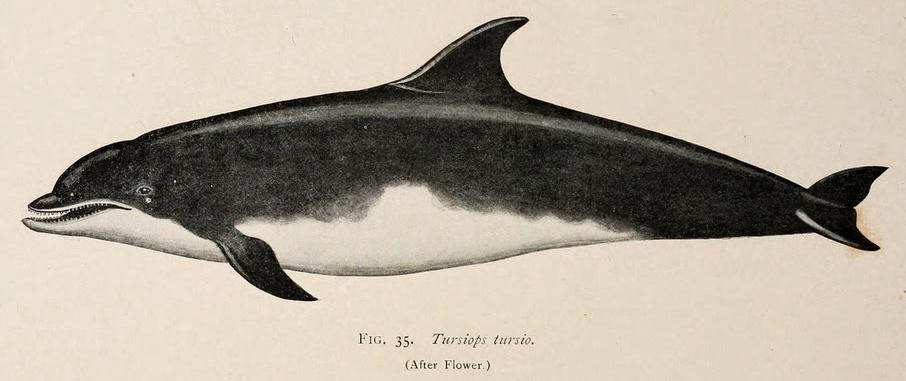
\includegraphics[width=\textwidth]{tursiops}
   	\small{Frank E. Beddard, A Book of Whales ($1900$)}
   \end{figure}
   
    \textbf{\textsc{ Rapport de stage de Master 2}}\\[1cm]
	
\textrm{\Large{Pierre-Louis}} \textsc{\Large{Stenger}}\\[1cm]

        \emph{Maîtres de stage} : \\
		
		\textrm{\large{Benoit}} \textsc{\large{Simon-Bouhet}}
		\& \\
		\textrm{\large{Hélène}} \textsc{\large{Labach}}


    \vfill

    % Bottom of the page
    {\large Janvier 2016 — Juin 2016}

  \end{center}
  \end{sffamily}
\end{titlepage}

% -------------------- Remerciements--------------------

\pagenumbering{roman} \setcounter{page}{1} 

\begin{center}
 \textsc{\LARGE Remerciements}\\[2cm]
\end{center}

Je voudrais en premier lieu te remercier chaleureusement Benoit, tout d'abord pour ce stage que tu as rendu possible, dans ce domaine pour lequel tu m'as fait prendre goût en écoutant tes cours de Génétique des Populations sur les bancs de la fac, mais aussi pour la pédagogie et la patience dont tu as fait preuve devant mes questions et mes interrogations chaque fois que ce fût nécessaire. Entre le méli-mélo de fichiers, les codes incorrects ou les heures de débuggages sur le Li-Cor, il en aura fallut de la patience ! Je n'aurai jamais autant appris en si peu de temps. Encore merci.
 
Un grand merci à toi Hélène, qui sans toi non plus, ce stage n'aurait pas pu ce réaliser. Malgré la distance tu as su être présente quand il le fallait, que cela soit par mail, téléphone ou Skype. Encore merci pour ces quelques jours passés sur Marseille où j'ai pu assister au déroulement du Workshop et rencontrer toutes ces personnes extraordinaires !

Encore un grand merci à vous deux.

Merci à Willy Dabin pour ses conseils très précieux, ainsi qu'à Fabien Demaret pour m'avoir permi de découper ces charmants bestiaux et fait découvrir les entrailles du vieux centre Océanographique de La Rochelle !

Merci à Éric et à Amélia qui ont pu me conseiller et m'aiguiller sur des questions de théorie génétique et d'informatique.

Merci aussi à Vanessa Becquet, Hélène Agogué et Martine Bréret qui ont su être là pour m'aider sur la plateforme technique de biologie moléculaire, mais aussi pour leur gentillesse et leurs conseils.

Un merci tout particulier à mes collègues stagiaires de bureau, et collègues doctorants: Alice et ses appels qui n'en finissaient pas (Et désolé pour la Clio sur le BonCoin haha !), Yann et son amour pour les phoques et le Nord (On va finir par y aller en vacances à force !), Mathilde l'accro au sport, Fanny et ses cookies si bons, Émeric qui nous a quitté pour aller se la couler douce à la NASA à L.A., Victor (on aura bien sué dans ce gymnase !), Antoine (Et ça pollue l'océan en perdant ses palmes ! Super session en tout cas !), et à tous les autres de LR qui se sont enkystés comme moi dans ce lieu ou il y fait bon vivre. À nos nombreuses pauses café, à tous nos gâteaux et nos soirées. Merci pour votre soutien et votre amitié.

Et enfin merci à mes parents, qui ont permis la réalisation de mes études, qui ont toujours étaient là pour moi et sans qui je n'aurais pas pu faire ce qui me plait aujourd'hui.

\newpage
\tableofcontents


\newpage
\listoffigures  % table des figures
\listoftables   % table des tableaux
\listof{enca}{Liste des encadrés}

\newpage

% -------------------- Description de la structure d'acceuil--------------------

\begin{center}
 \textsc{\LARGE Description de la structure d'accueil}\\[2cm]
\end{center}
\pagenumbering{arabic} \setcounter{page}{1} 
\addcontentsline{toc}{section}{Description de la structure d'accueil}

La structure d'accueil de ce stage fut le Centre d’Études Biologiques de Chizé qui est une unité mixte de recherche (UMR 7372 – CNRS (Centre National de Recherche Scientifique) – Université de La Rochelle). Ce centre est composé de trois équipes de recherche. Ce stage a été fait au sein de l’équipe « Prédateurs marins » qui recherche notamment les conséquences de la variabilité climatique et océanique sur la distribution des ressources ainsi que sur la démographie des prédateurs marins.

Le laboratoire d'accueil fût LIENSs (LIttoral ENvironnement et Sociétés - UMR 7266) est une Unité Mixte de Recherche (CNRS / Université de La Rochelle) qui met en avant sa pluridisciplinarité afin de répondre aux enjeux du développement durable en lien avec le littoral. C'est ici que j'ai pu réaliser toutes les analyses génétiques (en laboratoire et sur logiciels) avec le Dr Benoit Simon-Bouhet.

~~\\

Le second organisme avec le quel j'ai pu collaborer est le GIS3M (Groupement d’Intérêt Scientifique pour les Mammifères Marins de Méditerranée) qui est une association crée le 7 août 2007. Actuellement situé à Sausset-les-Pins dans les Bouches-du-Rhône, elle compte 23 membres depuis 2015, dont la présidente est le Dr Hélène Labach.

L’objectif du GIS3M est de favoriser l'association des compétences dans le domaine de la recherche sur les mammifères marins de Méditerranée. Notamment en permettant de rassembler les chercheurs et spécialistes pluridisciplinaires, ainsi que d'apporter une aide matérielle et financière autour de projets de recherche collaboratifs.

Je n'ai pas pu être sur le site de l'association du GIS3M à Sausset-les-Pins, mais j'ai eu l'occasion de me déplacer sur Marseille du 29 novembre au 3 décembre 2015 afin de pouvoir rencontrer les membres de l'association, de participer à une réunion des partenaires du projet GDEGeM (Grand Dauphin Etude et Gestion en Méditerranée) dans lequel s'est inscrit ce stage. Cette réunion s'est déroulée à la DREAL (Direction Régionale de l'Environnement, de l'Aménagement et du Logement) de Marseille. J'ai aussi pu assister et aider à la mise en place de l'``International Workshop Bottlenose dolphin conservation and monitoring in the North-Western Mediterranean Sea'' qui s'est déroulé à la Villa Méditerranée de Marseille les 1 et 2 décembre.


\newpage

\title{{\Huge État de l'art}\\[3pc]Séquençage haut débit et inférences de la structure de populations : perspectives nouvelles et limites}
\author{Pierre-Louis \textsc{Stenger}}
\date{}

\frontmatter

\maketitle 

~~\\
\textbf{Mots clés:} \emph{NGS, Population, Génétique, Conservation, Structure de population}
~~\\

\newpage

\mainmatter

%\pagenumbering{arabic} \setcounter{page}{1} 

\begin {bibunit} [newbst]
\addcontentsline{toc}{section}{État de l'art} 
Le taux d'extinction des espèces animales à la surface du globe est actuellement 1000 fois supérieur au taux normal supposé \citep{pimm2014aa}. Les conséquences des actions anthropiques sur l'environnement en général et sur la biodiversité en particulier sont telles que certains auteurs n'hésitent pas à parler d'anthropocène pour caractériser l'ère géologique dans laquelle l'Homme semble avoir fait entrer la Terre depuis la fin du XIX\ieme{}~siècle \citep{crutzen23ff}. Dans ce contexte, les efforts de protection de la biodiversité et de conservation des espèces sont plus que jamais d'actualité.\footnote{Google Scholar indique par exemple que 398 articles publiés en 2015 contiennent, dans leur titre, l'expression ``biodiversity conservation''.} Depuis le milieu du XX\ieme{}~siècle, la prise de conscience de l'impact des activités humaines sur le milieu marin a conduit le législateur à créer des zones de protection en mer comme avec le double objectif de maintenir les activités humaines tout en protégeant la biodiversité \citep{frost2016} L'efficacité des aires marines protégées repose sur la détermination préalable de la structure des populations, qui est très difficile à déterminer en milieu marin \citep{Jonsson2016} pour deux raisons principales:

\begin{enumerate}
	\item la plupart des espèces sont difficiles voire impossibles à observer ou à marquer. C'est par exemple le cas pour les mammifères marins dont 23\% des espèces sont pourtant actuellement menacées d'extinction \citep{schipper2008status}.
	\item l'extrême fécondité de certaines espèces (par exemple \emph{Ostrea virginica} peut relarguer de 15 à plus de 110 millions de gamètes dans le milieu marin, \citealp{galtsoff1930fecundity}) rend l'inférence de la connectivité, et donc de la structure de populations, très difficile \citep{gagnaire2015aa}.
\end{enumerate}

Pourtant, l'inférence de la structure des populations est critique pour la mise en place de mesures de protection adaptées. Par exemple, une analyse de risque a montré que dans l'Atlantique Nord-Est, le niveau de captures accidentelles subit par le dauphin commun \emph{Delphinus delphis} n'est pas supportable sous l'hypothèse d'une population structurée en 2 stocks, l'un néritique et l'autre océanique \citep{Mannocci2012}. La détermination précise de la structure de population d'une espèce d'intérêt est donc une question centrale dans le domaine de la conservation. Lorsqu'il est impossible de déterminer la structure des populations par des méthodes directes, le recours à des méthodes indirectes doit alors être envisagé. Ainsi, de nombreuses approches sont couramment utilisées pour l'étude de populations naturelles, notamment en milieu marin comme: 
\begin{itemize}
	\item l'étude de traceurs écologiques : isotopes stables du carbone, de l'azote et du souffre, acides gras, métaux lourds \citep{newman2000stock},
	\item l'analyse des contenus stomacaux \citep{spitz2006diet, spitz2011prey} ou encore,
	\item l'utilisation de marqueurs moléculaires (allozymes, RAPD, ADN mitochondrial, microsatellites, SNP, etc) \citep{pogson1995genetic, huang2000analysis}.
\end{itemize}

Les études de génétique des populations sont extrêmement utiles pour inférer la structure des populations car les évènements démographiques et évolutifs laissent des traces dans l'ADN des populations. À l'échelle micro-évolutive, il est généralement admis que le niveau de diversité génétique d'une population est proportionnel à sa taille efficace\footnote{La taille efficace cst le nombre d'individus d'une population idéale pour lequel on aurait un degré de dérive génétique équivalent à celui de la population réelle. } \citep[voir][pour une discussion à ce sujet]{bazin2006population, MK06a, Ey06}. Un prélèvement ponctuel chez quelques individus d'une population permet alors d'aborder, entre autres, des questions relatives à la taille actuelle et passée des populations \citep{tajima1989effect, beerli2001maximum}, à leurs limites géographiques \citep{franccois2010spatially, guillot2012} et à leur connectivité grâce à l'inférence des taux de migrations entre populations \citep{wilson2003bayesian}. Toutefois, comme pour toutes les méthodes indirectes, les outils moléculaires présentent un certain nombre de limites. En effet, les marqueurs classiques tels que l'ADN mitochondrial ou les microsatellites ne permettent que rarement l'accès aux temps courts (quelques générations, du fait de la lenteur de l'apparition de mutations, \citealp{drake1998rates}) et à l'échelle locale. En outre, la puissance statistique augmentant avec le nombre de marqueurs \citep{waples1998separating, latch2006relative}, les inférences réalisées avec les marqueurs classiques (généralement utilisés en faible nombre) sont parfois peu concluantes. 

\begin{enca}
\caption{Les forces évolutives}\label{Forces}
\onehalfspacing
	Les forces évolutives sont des processus qui modifient les fréquences alléliques observées dans les populations au fil des générations. Elles sont au nombre de 4 :
\begin{description}
	\item[Mutation] : changement accidentel du patrimoine génétique d'un individu. À l'échelle de l'espèce, c'est une source d'innovation qui permet d'augmenter la diversité génétique globale.
	\item[Dérive génétique] : fluctuation aléatoire des fréquences alléliques au fil des générations liée à un effet d'échantillonnage. Le pool de gènes d'une population à la génération $g$ est issu de tirages aléatoires parmi le pool de gènes de la population à la génération $g-1$. L'amplitude des fluctuations de fréquences alléliques est inversement proportionnelle à la taille de la population. La dérive génétique peut donc conduire à une perte de diversité genétique en ramenant à 0 la fréquence de certains allèles.
	\item[Migration] : échange de gènes entres populations distinctes. À chaque génération, une fraction du pool génique d'une population peut provenir d'une autre population. Cette force évolutive tend à homogénéiser les pools de gènes des populations échangeant des migrants et à limiter les risques de perte de diversite génétique.
	\item[Sélection] : une population est soumise à sélection si la capacité des individus à produire des descendants fertiles est influencée par leur génotype. Certaines formes de sélection vont favoriser un allèle particulier dont la fréquence augmentera au détriment des autres. Dans ce cas, comme pour la dérive génétique, la sélection tend à diminuer la diversité génétique. D'autres formes de sélection vont au contraire permettre le maintien de plusieurs formes alléliques. Dans ce cas, comme pour la migration, la sélection limite les risques de perte de diversité génétique.
\end{description}
\end{enca}

Ainsi, l'étude de l'isolement par la distance (ou IBD : Isolation By Distance) est une méthode couramment utilisée pour étudier la structure des populations. Elle permet de mesurer l'augmentation de la différenciation génétique avec un accroissement des distances géographiques entre les populations \citep{rousset1997genetic} ou les individus \citep{rousset2000genetic} quand la dispersion spatiale est limitée. La détection d'IBD suppose (i) que la dérive génétique conduise à des niveaux de différenciation génétique suffisants entre populations et (ii) que la migration entre populations soit limitée afin d'éviter l'homogénéisation trop importante des stocks génétiques (voir encadré~\ref{Forces}). Si la dérive génétique est trop faible, la dispersion ne peut pas être inférée grâce à un modèle reposant sur l'équilibre migration/dérive \citep{gagnaire2015aa}. Puisque de nombreuses espèces marines présentent des tailles de populations très importantes et des capacités de dispersion élevées grâce à un stade de vie larvaire \citep[e.g. chez les poissons et invertébrés][]{dewoody2000microsatellite, mccusker2010positive}, la méthode de l'IBD est souvent inutilisable avec les marqueurs classiques qui présentent, dans ces conditions, des niveaux de différenciation génétiques faibles \citep{selkoe2011marine}.

Les analyses bayésiennes de clustering sont une autre famille de méthodes permettant d'inférer la structure des populations. Implémentées dans différents logiciels (e.g. \texttt{Structure}, \citet{pritchard2000inference}, \texttt{TESS}, \citet{franccois2010spatially}, \texttt{Geneland}, \citet{guillot2012}), elles permettent de détecter les discontinuités génétiques (donc les limites entre stocks génétiques distincts) et les migrants \citep{broquet2009molecular}. Ces méthodes déterminent tout d'abord le nombre de populations le plus vraissemblable compte tenu de l'information génétique disponible (et pour certains logiciels, des coordonnées géographiques des individus étudiés) et calculent ensuite, pour chaque individu échantillonné, la probabilité d'assignation à chacune des populations inférées \citep{pritchard2000inference, corander2003bayesian}. Pour être précises, ces approches requièrent une forte densité d'échantillonnage sur une large échelle géographique. Leur intérêt est donc limité pour les espèces dont la distribution géographique est mal documentée \citep{gagnaire2015aa}, ce qui est encore aujourd'hui fréquent en milieu marin \citep{novak2016predictive}.

Outre les difficultés d'inférence de la structure des populations liées aux taux d'évolution des marqueurs décrites ci-dessus, la prise en compte de la sélection est un autre problème difficile à aborder à l'aide des marqueurs génétiques classiques. Puisque la sélection peut laisser dans les populations des traces comparables à celles d'autres forces évolutives (voir encadré~\ref{Forces}) ou à certains régimes de reproduction (consanguinité notamment), les généticiens des populations font généralement abstraction de la sélection en utilisant des marqueurs neutres \citep{bazin2006population}. Or, il est maintenant admis que la préservation des adaptations locales est un enjeu de conservation majeur \citep{hallfors2015addressing}. Elle est d'ailleurs au c\oe ur de la notion d'ESU : Evolutionary Significant Units \citep{crandall2000}.\\

Dans ce contexte, la génomique des populations\footnote{C'est l'étude, à l'échelle des populations, de l'information génétique répartie dans l'ensemble du génome des individus. La génomique des populations permet d'étudier conjointement des dizaines ou des centaines de milliers de \emph{loci} et non plus seulement quelques dizaines.} ouvre de nouvelles perspectives prometteuses en terme de conservation \citep{shafer2015genomics, garner2015genomics, luikart2003power}. En effet, depuis le début des années 2000, de nouvelles technologies de séquençage de l'ADN à très haut débit\footnote{NGS : Next Generation Sequencing} apparaissent et permettent de générer de très grandes quantités d'informations génétiques à moindre coût. Les technologies de séquençage sont nombreuses et évoluent très vite. Citons, parmi les principales, la technique de pyroséquençage 454 (société Roche, avec les appareils GS Junior System, et GS FLX+ System \citep{GSFLX}), la technique d'Illumina (société Solexa avec les appareils HiSeq System, Genome analyser Ilx ou encore MySeq \citep{illumina}), la technique de Life Technologies (société Applied Biosystems avec les appareils SOLID 5500 System \citep{shokralla2012next}) ou encore la technique Ion Torrent de la même société (Life Technologies, avec les appareils Personal Genome Machine et Proton \citep{iontorrent}). Et depuis 2012, une nouvelle génération de séquenceur encore plus performant arrive sur le marché (e.g. Helicos Genetic Analysis System, PacBio RS, GridION System et MinION \citep{mikheyev2014first}). 

La génération rapide de centaines de millions de séquences d'ADN s'est accompagnée d'une chute vertigineuse des coûts et des temps de séquençage : en l'espace de 10 ans, le prix de séquençage d'un génome humain a ainsi été divisé par plus de $100\,000$ (figure~\ref{fig:moore}). Le prix d'un génome complet approchant les $1\,000$ dollars \citep{hayden20141}, la génération d'information génomique n'est plus réservée à quelques organismes modèles \citep{ekblom2014field, shafer2015genomics}. En outre le développement de méthodes NGS ciblant en priorité des zones d'intérêt du génome (i.e. les zones présentant de fortes densités de SNPs\footnote{Single Nuclear Polymorphism : polymorphisme d'un seul nucléotide}), les études génomiques à l'échelle des populations sont maintenant envisageables \citep{davey2010radseq}.

\begin{knitrout}
\definecolor{shadecolor}{rgb}{0.969, 0.969, 0.969}\color{fgcolor}\begin{figure}[htpb]

{\centering 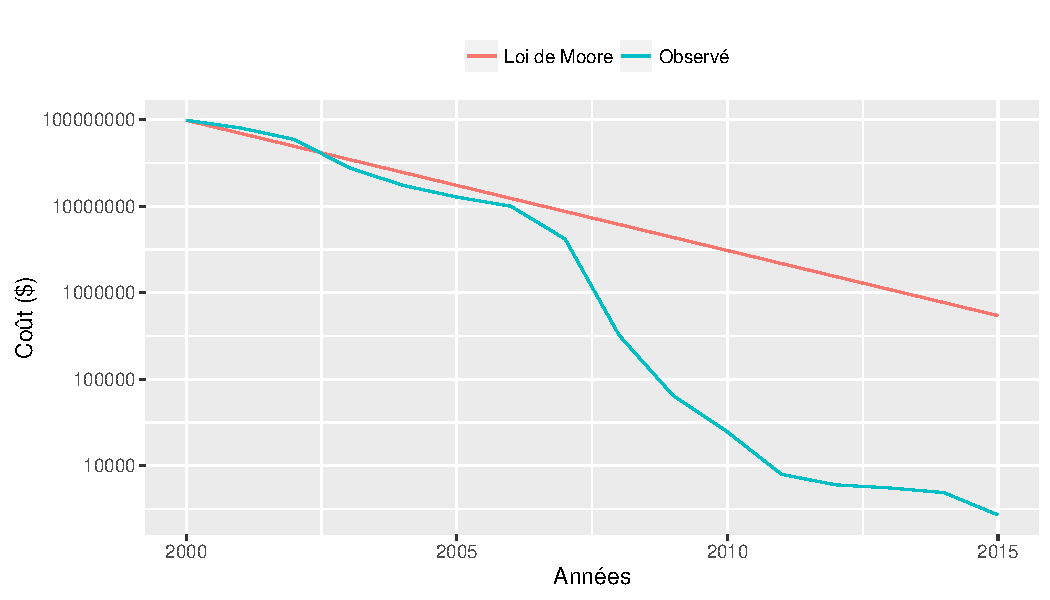
\includegraphics[width=15cm,height=8.6cm]{figure/moore-1} 

}

\caption[Évolution du coût de séquençage d'un génome humain]{Évolution du coût de séquençage d'un génome humain (données du NHGRI Genome Sequencing Program, www.genome.gov/sequencingcostsdata)}\label{fig:moore}
\end{figure}


\end{knitrout}

L'utilisation de marqueurs en grand nombre (de quelques centaines à plusieurs centaines de milliers) augmente fortement la puissance statistique des tests utilisés \citep{waples1998separating, gagnaire2015aa}, ce qui permet par exemple d'inférer la structure des populations à très fine échelle spatiale et temporelle \citep{szulkin2016population, mccormack2013next}. À titre d'exemple, le genotypage de nombreux SNPs chez quatre espèces de poissons commerciaux a permis de décrire la structure des populations à une échelle géographique très fine, jusqu'alors inaccessible \citep{martinsohn2009fishpoptrace, shafer2015genomics}. Ces progrès ont permis de détecter des erreurs d'étiquetage sur les étals ou des fraudes concernant l'origine des poissons, et donc la mise en application directe de mesures de protection adaptées \citep{martinsohn2009fishpoptrace}.
Ces nouvelles approches permettent en outre d'accéder aux zones du génome subissant la sélection et offrent donc l'opportunité de détecter la mise en place d'adaptations locales par les populations \citep{stapley2010adaptation} ce qui est par\-ti\-cu\-lière\-ment utile dans un contexte de conservation \citep{steiner2013conservation}. Ainsi, la méthode des ``loci outliers'' permettant de détecter des zones du génome potentiellement sous sélection (voir encadré~\ref{outlier}) est souvent considérée comme l'une des plus grandes avancées récentes dans le domaine de la conservation \citep{funk2012harnessing, mcmahon2014and, shafer2015genomics}.

\begin{enca}
	\caption{Les loci outlier}\label{outlier}
    Le $F_\text{ST}$ est un indice de fixation permettant d'estimer le niveau de différenciation entre 2 populations grâce aux fréquences alléliques observées dans ces populations. Pour un niveau d'hétérozygotie donné à un locus précis, il est possible de calculer la gamme de variation attendue du $F_\text{ST}$ sous l'hypothèse de neutralité. Les loci qui présentent des valeurs de $F_\text{ST}$ en dehors de cette gamme sont appelés loci outlier. Ils peuvent être sous sélection positive ou sélection balancée.


{\centering 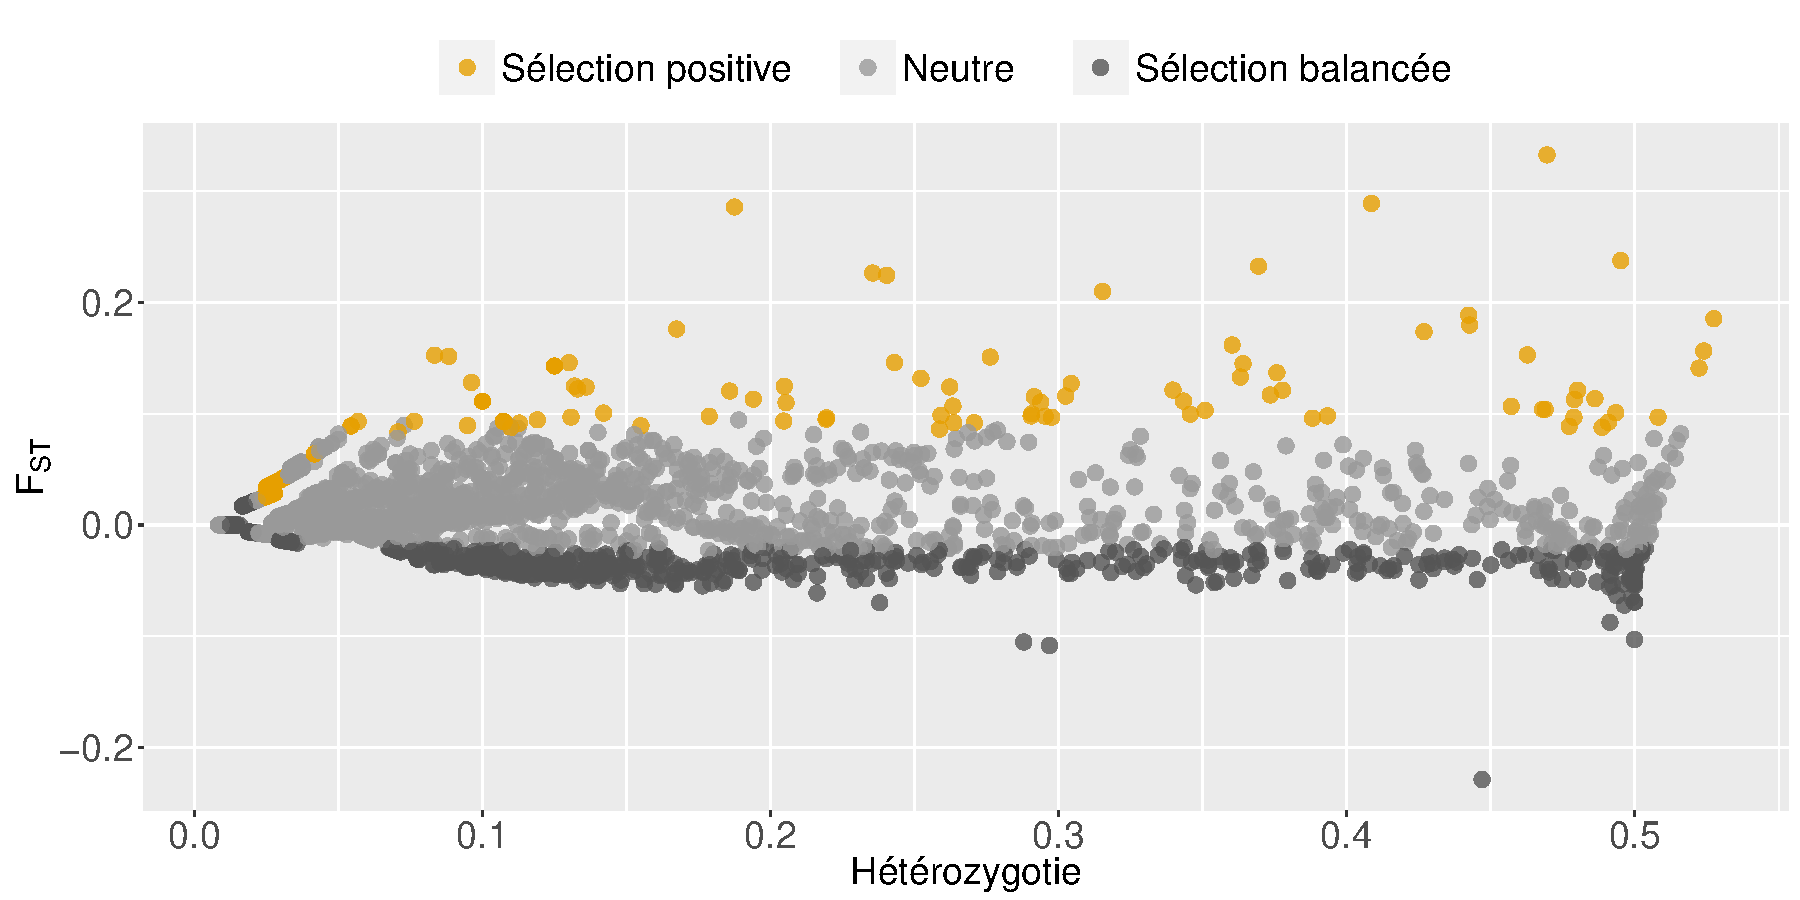
\includegraphics[width=14cm,height=7cm]{figure/lositan-1} 

}



		
\end{enca}

L'utilisation des NGS présentent néanmoins un certain nombre de limites. La qualité et la quantité d'ADN nécessaire pour mettre en oeuvre les NGS est importante \cite{davey2011genome}. En effet, les organismes de toute petite taille \citep{baily1992detection} ou pour lesquels l'ADN est dégradé comme pour les échantillons issus d'individus échoués (cétacés) \citep{taberlet2012towards, templeton2013dna} apportent des difficultés liées aux quantités et à la qualité d'ADN nécessaire pour les méthodes de séquençage par NGS. Au laboratoire, les protocoles sont beaucoup plus longs et complexes qu'avec les méthodes classiques. Les risques de biais méthodologiques sont donc nombreux \citep[voir par exemple][]{bonin2004aa, baird2008aa, peterson2012double, hohenlohe2012extensive, niu2010artificial, gomez2009systematic,haas2011chimeric} et les erreurs de séquençage sont également plus fréquentes qu'avec les méthodes classiques \citep{mastretta2015restriction, shendure2008next}.

Les NGS présentent aussi des difficultés liées à la puissance de calcul nécessaire au traitement de ces données très abondantes. Le temps de calcul ou le nombre de processeurs nécessaires pour le nettoyage des données et l'assemblage d'un génome est variable selon la taille des génomes. En outre, ces techniques présentent des difficultés liées aux outils et méthodes d'analyse statistique.  Sur le long terme, il sera essentiel de développer une gamme de protocoles de laboratoire comme celle proposé par \citet{zielinski2014development} et \citet{lighten2014aa}, car ces méthodes sont encore coûteuses pour une utilisation en routine. De plus, les pipelines d'analyses sont encore en développement pour la plupart des techniques de NGS \citep{lighten2014aa} ce qui ne facilite pas leur utilisation et il n'y a pas encore de véritable standard. Néanmoins, quelques pipelines d'analyses semblent vouloir commencer à s'imposer comme le logiciel Genome Analysis Toolkit du Broad Institute au MIT. Il s'agit d'une bibliothèque logicielle structurée qui permet d'utiliser efficacement des outils d'analyse avec des données issues des NGS \citep{lam2012detecting}. Des ordinateurs à haute performance sont généralement nécessaires pour le stockage et l'analyse de ces données \citep{shafer2015genomics, garner2015genomics} et l'extraction des données est parfois problématiques. Par exemple, un fichier SFF (Standard Flowgram File) est créé en sortie standard de la technologie 454 (Fichier binaire qui est humainement illisible \citealp{peyretaillade2011extreme}), et il faut alors un exécutable particulier pour les décoder. Il y a donc un réel besoin de bio-informaticiens ayant la double compétence génétique des populations/programmation.

Malgré ces nombreuses difficultés, la puissance des NGS permet aujourd'hui d'envisager des avancées rapides en terme de conservation \citep{shafer2015genomics}. L'identification de structure de populations à très fine échelle \citep{o2015rare} ou l'obtention de très grandes quantité de données génétiques sur des espèces difficiles à observer et échantilloner sur le terrain (e.g. le grand dauphin \emph{Tursiops truncatus}, \citealp{schipper2008status}) sont autant de facteurs clés pour l'identification d'ESU (Evolutionary Significant Unit, \citealp{ryder1986species}) et la mise en place de MU (Management Unit, \citealp{hawkins2016fisheries}) indispensables à la conservation des espèces \citep{casiraghi2016}.


\newpage
	\begin{otherlanguage}{english}
		\singlespacing
		\begin{multicols}{2}[]
		\putbib [BibliographieEA]
	\end{multicols}
\end{otherlanguage}

\end {bibunit}


\newpage


\begin {bibunit} [newbst]
\addcontentsline{toc}{section}{Rapport}
\section{Introduction}

Dans les eaux méditerranéennes françaises, les aires marines protégées incluant 2 parcs nationaux, 1 parc marin, 36 (ZSC) Zones Spéciales de Conservation ou ZPS (Zones de Protection Spéciales) et 5 ASPIM (Aire Spécialement Protégée d’Importance Méditerranéenne), couvrent 34\% de la ZEE (Zone Économique Exclusive) \citep{workshop}. Ce réseau de protection est justifié par le fait que la mer Méditerranée est un point chaud de la biodiversité marine \citep{coll2010biodiversity}. Néanmoins, les tendances temporelles indiquent que la surexploitation et que la destruction de l'habitat ont été les principaux facteurs humains impliquants des changements historiques dans la biodiversité \citep{danovaro2003pollution, coll2010biodiversity}. Tous ces impacts devraient croître en importance à l'avenir, en particulier avec le changement climatique et la dégradation de l'habitat \citep{coll2012mediterranean}. 

L’inférence de la structure des populations est capitale pour la mise en place de mesures de protection adaptées \citep{hoelzel1998genetic}, ainsi que pour adapter les plans de gestion des aires marines protégées \citep{MPA}. Surtout dans un monde où les espèces évoluent et s'adaptent dans un milieu changeant.

Les populations sont aussi définies comme des unités d'organismes avec des dynamiques autonomes et le recrutement d'individus permettant des métissages \citep{krutzen2004population}. Définir les limites d'une population donnée est une condition préalable non seulement à des fins de gestion tels que la définition des unités significatives de l'évolution (ESU\footnote{Une ESU est une population d'organismes qui est considérée comme distincte à des fins de conservation .}) \citep{hoelzel1998genetic, carnabuci2016} ou dans le management de ces unités (MU\footnote{Les MU sont définis comme des populations qui ont des fréquences différentes d'allèles , mais ne montrent pas nécessairement des différences fixes entre les populations}) \citep{ryder1986species, hawkins2016fisheries}, mais aussi pour étudier l'évolution de la structure au sein d'une population \citep{carnabuci2016}. Cependant, la détermination préalable de la structure des populations est très difficile à déterminer en milieu marin \citep{Jonsson2016}. De plus, 23\% des espèces de mammifères marins sont actuellement menacées d’extinction \citep{schipper2008status}. 

Cependant, en dépit de leur capacité de nage développées, les mammifères marins montrent souvent une structure de population à petite échelle, bien que la mesure varie selon les espèces \citep{hoelzel2002low}. Dans cette étude, nous étudions la structure de la population pour une espèce marine sociale avec une grande mobilité: le grand dauphin \emph{Tursiops truncatus}, Montagu, 1821.

Bien que les \emph{Tursiops truncatus} sont parmi les cétacés les plus connus dans la Mer Méditerranée, les études de ce cétacé n'ont commencé qu'à la fin des années $1980$ \citep{bearzi2009ecology}. Les enjeux de conservation sont pourtant importants pour cette espèce patrimoniale. 

Un réel besoin de connaissances sur leur structure de population se fait ressentir. De plus, ces dauphins ont été qualifiés comme ``vulnérable'' selon l'Union Internationale pour la Conservation de la Nature selon les critères de la Liste rouge \citep{bearzi2006common}. Cette espèce a aussi été inscrite sur l'annexe II de la directive Habitats de l'UE dans la région méditerranéenne \citep{Laran2016}. L'objectif général est de maintenir (ou de restaurer) l'espèce à un état de conservation favorable \citep{evans2004monitoring}. Cela nécessite des informations sur la structure des populations.

L'inférence de leur structure de population \emph{via} l'utilisation de marqueurs génétiques comme les microsatellites et mitochondriaux s'avère être pertinent pour ce cas d'étude \citep{natoli2004molecular}. En effet, malgré l'absence de barrière environnementales au flux de gènes, les processus environnementaux historiques et spécialisations écologiques peuvent conduire à une différenciation génétique chez les animaux très mobiles \citep{natoli2005habitat, louis2014}. Les microsatellites sont des marqueurs d'ADN\footnote{Acide désoxyribonucléique} nucléaires avec une héridité bi-parentale \citep{jarne1996microsatellites}. Les microsatellites sont des séquences nucléotidiques courtes de deux à quatre paires de bases répétées en tandem, largement intercalés dans le génome eucaryote\footnote{Organismes uni- ou pluricellulaires qui se caractérisent par la présence d'un noyau} dans les parties non codantes \citep{estoup2002homoplasy}. Les microsatellites sont des marqueurs hautement informatifs car ils ont un polymorphisme\footnote{Désigne la coexistence de plusieurs allèles pour un gène ou locus donné} extrêmement variable et sont généralement considérés comme neutres (ne subissant pas la sélection) \citep{jarne1996microsatellites}. L'ADN mitochondrial est une molécule circulaire et haploïde \citep{avise1987intraspecific}. Chez les mammifères, il est maternellement hérité et non soumis à la recombinaison. L'absence de recombinaison permet la détection d'événements évolutifs passés tels que les migrations, les goulots d'étranglement, les isolements de la population dans les différentes lignées maternelles \citep{avise1987intraspecific, excoffier1992analysis}. L'analyse combinée de ces marqueurs est particulièrement utile dans les espèces ayant un comportement social complexe \citep{natoli2004molecular}. En raison de mode d'évolution contrastés suivant leur héritage, il est possible d'avoir un aperçu de la structure des espèces \citep{natoli2005habitat}.

Ainsi, un échantillonnage de tissus d'individus trouvés échoués sur les côtes méditerranéennes ainsi que l'obtention de biopsies réalisées lors de campagnes en mer ont permis d'obtenir un jeu de données d'individus des côtes languedociennes, de Corse et d’Italie. Les données générées lors de cette étude ont été analysées conjointement avec des données générées par Marie Louis lors de son doctorat \citep{phdLouis2014}, notamment celles concernant la Méditerranée et la façade Atlantique de la Péninsule Ibérique. Les inférences de structure de populations ont été réalisées sur la base de ce jeu de données étendu. Pour caractériser ces populations, des indices de diversité génétique ont été calculés pour les données microsatellites et mitochondriales.

Ces résultats permettront d'apporter de nouvelles informations sur la distribution et la structuration de cette espèce de cétacé en Mer Méditerranée. Ils aideront donc à la prise de décisions politiques pour la protection de cette espèce, et par conséquent, sur les écosystèmes englobés dans leurs habitats.


\section{Matériel et méthodes} 

\subsection{Collecte des échantillons} 
Au cours de cette étude, 122 échantillons de tissus (peau, $N= 60$, muscle, $N= 37$, rein, $N= 21$, foie, $N= 1$, gencive, $N= 3$) issus de 67 individus des côtes languedociennes, de Corse et d'Italie (voir figure~\ref{fig:concentration}) ont été analysés. Ces échantillons sont en partie issus de la banque de réseau national d'échouage français ($N= 46$, individus échoués entre 2001 et 2015) géré par l'Unité Mixte de Recherche PELAGIS (UMS 3462) et d'une part issus de programmes de biopsies ($N= 16$, biopsies collectées par l'association GIS3M (Groupement d'Intérêt Scientifique pour les Mammifères Marins de Méditerranée), l'association GECEM (Groupe d'Etude des Cétacés de Méditerranée) et l'association BREACH (Des voiles pour les cétacés, étudier, protéger et connaitre les mammifères marins aux Antilles et en Méditerranée). Enfin, 5 échantillons d'individus échoués en Italie ont été fournis par le Dr Marco Ballardini\footnote{MSc, Sezione di Medicina Legale e Scienze Forensi A. Fornari, via Forlanini 12, 27100 Pavia}. La plupart des échantillons est conservée dans l'éthanol (70\%) et les biopsies les plus récentes ont été congelées. Pour chaque échantillon, un morceau de tissu de 0.5 cm$^3$ a été prélevé en vue des extractions d'ADN.

\begin{figure}[htbp]
	\centering
		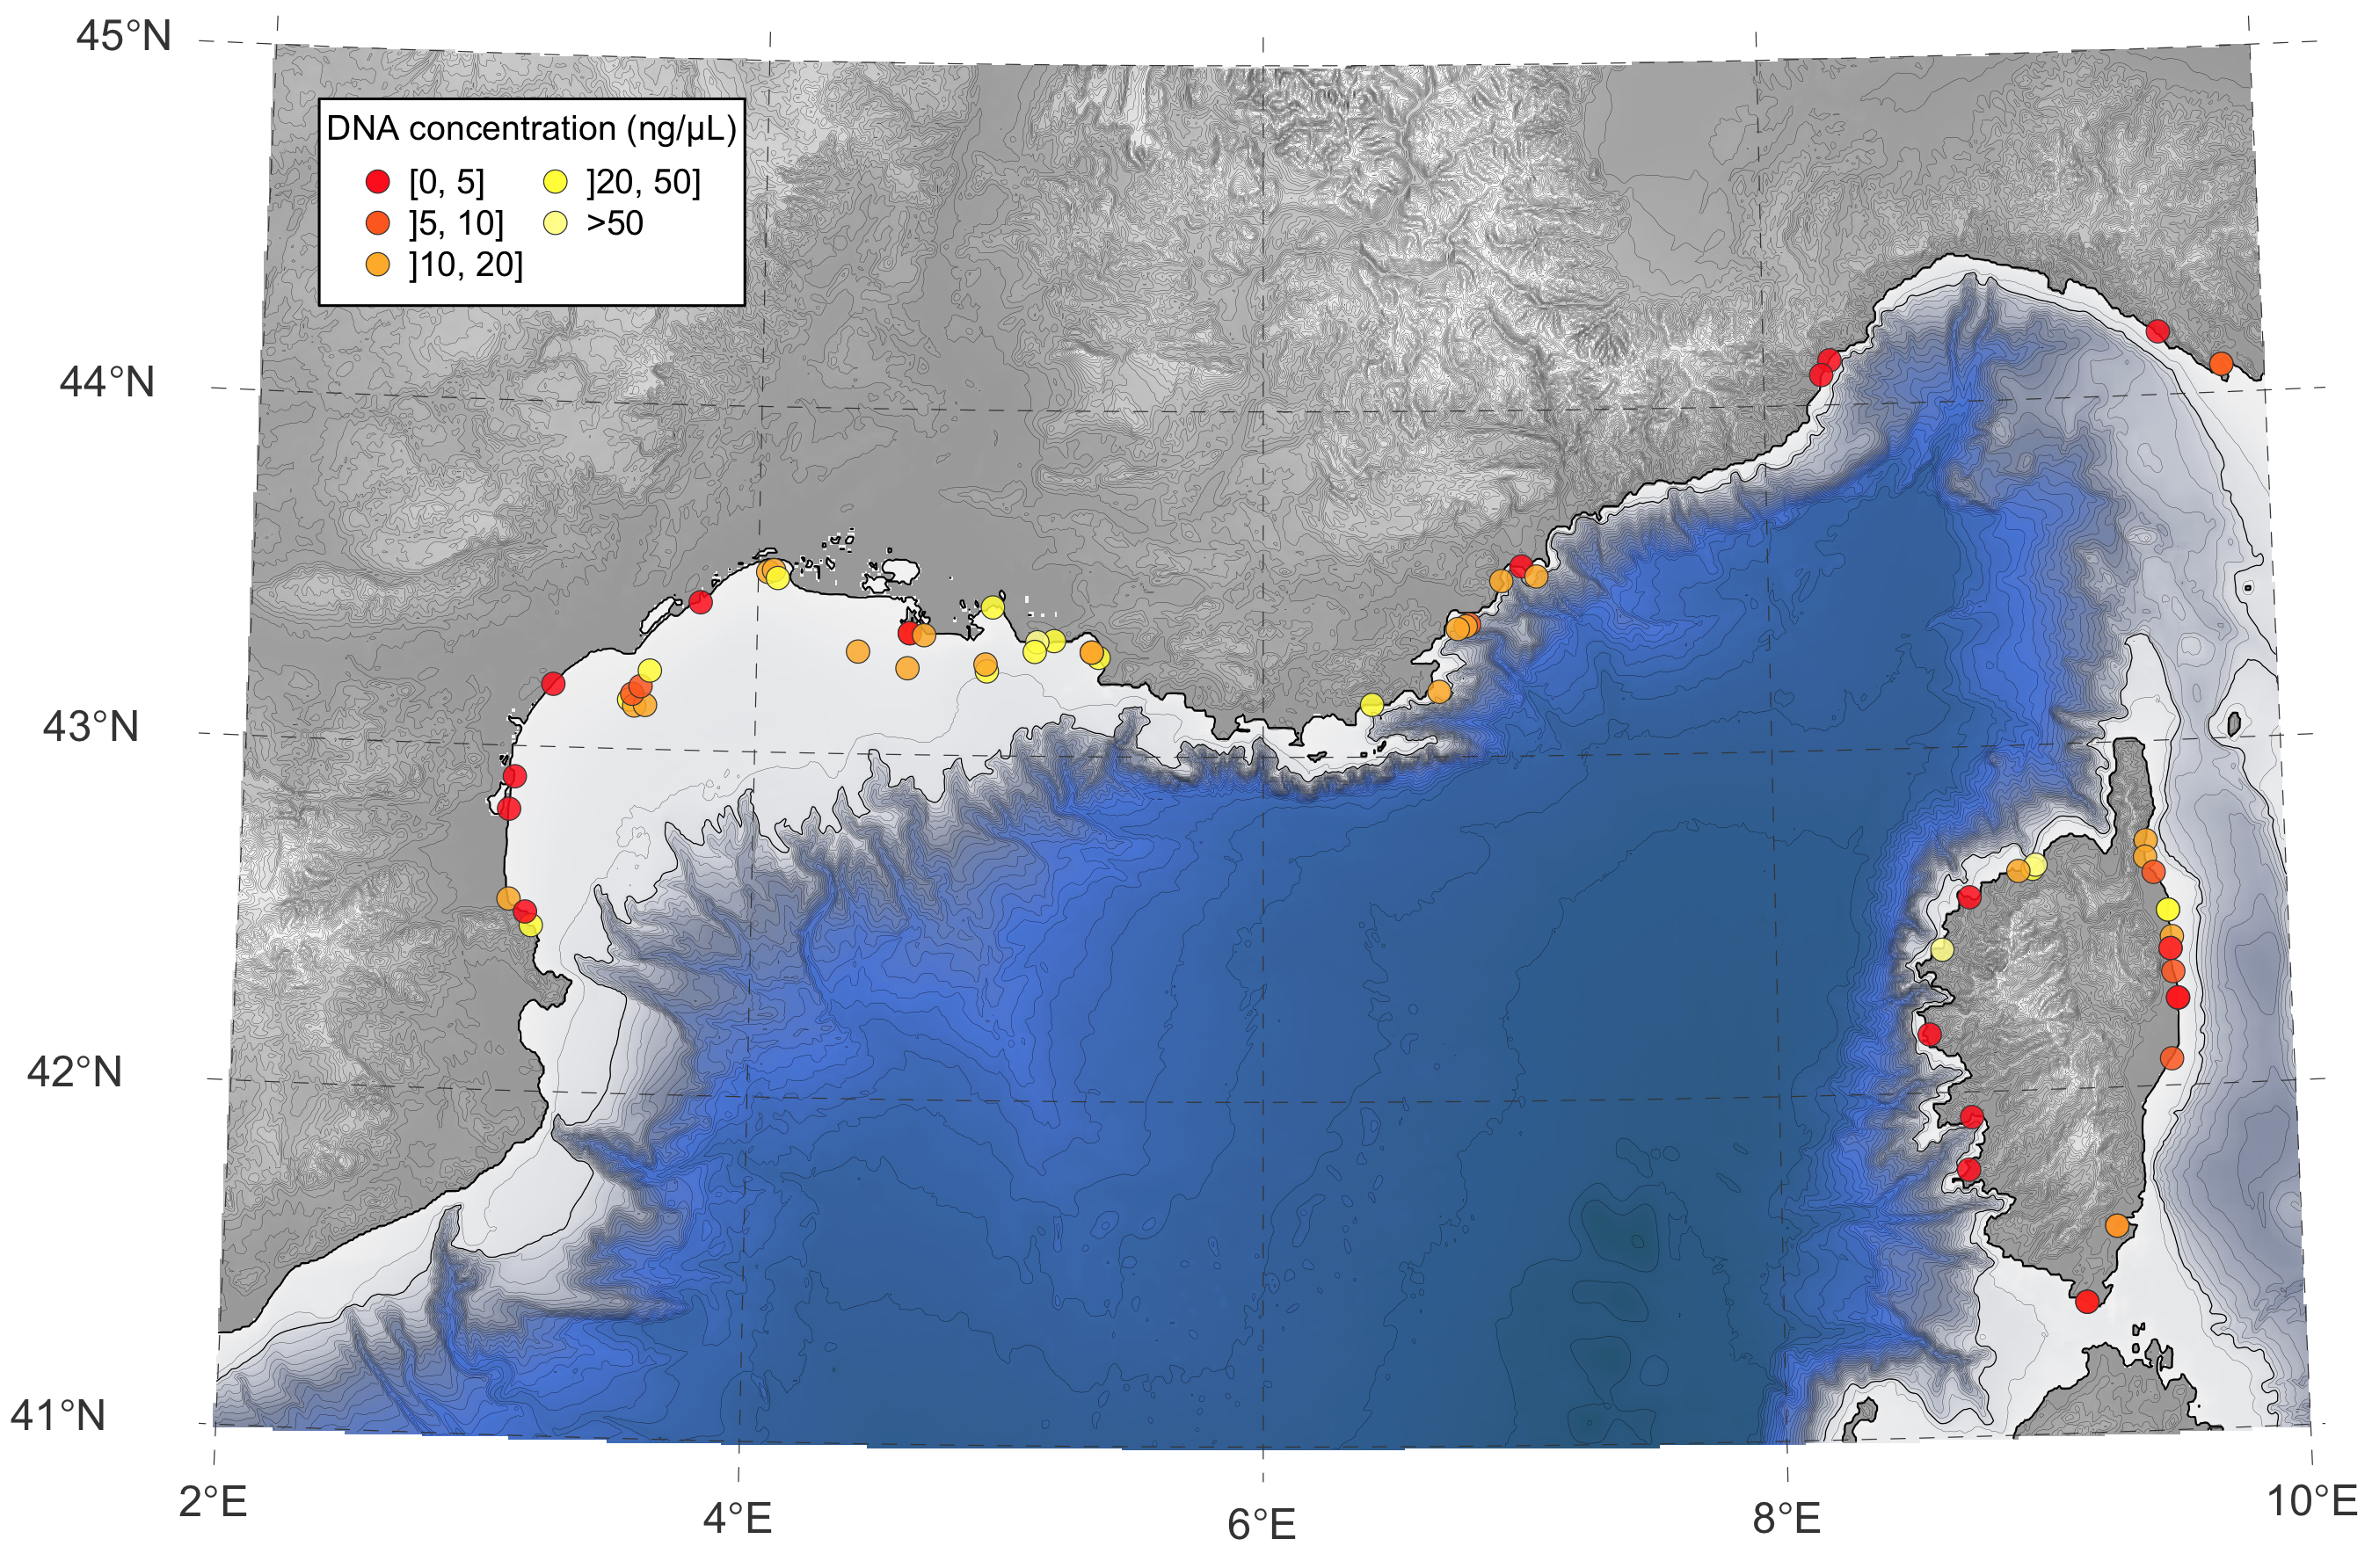
\includegraphics[width=\textwidth]{concentrations.png}
	\caption{Localisation des échantillons et concentrations d'ADN obtenues à l'issue des extractions}
	\label{fig:concentration}
\end{figure}


\subsection{Extractions d'ADN}
Pour certains échantillons, plusieurs extractions d'ADN ont été faites afin d'augmenter les quantités d'ADN disponibles pour la suite du protocole. Au total, 138 extractions d'ADN ont été réalisées à l'aide d'un kit NucleoSpin\textregistered{} Tissue (Macherey Nagel). Les échantillons sont découpés au scalpel et soumis à une lyse tissulaire en présence de protéinase K à 56ºC pendant 12 à 15 heures. Après un passage à 70ºC pendant 10 minutes, les échantillons sont placés sur une colonne contenant une membrane de silice à laquelle les acides nucléiques se fixent. Plusieurs étapes de rinçage (par ajout de tampons et centrifugation) permettent d'éliminer les résidus cellulaires. Enfin, les ADN sont récupérés grâce à 2 étapes de centrifugation successives après ajout de 100$\mu$L de tampon d'élution qui permet aux acides nucléiques de se décrocher de la membrane. Pour chaque échantillon, la concentration d'ADN a ensuite été mesurée par spectrophotométrie à l'aide d'un Nanodrop2000.

\subsection{Sexage}
Le sexage des \emph{Tursiops truncatus} a été effectué selon le protocole décrit par \citet{rosel2003pcr}. Un fragment du chromosome X et un fragment du chromosome Y sont amplifiés par PCR (Réaction de Polymérisation en Chaîne). Les 2 fragments d'ADN ciblés ayant des tailles différentes, il est possible de les distinguer visuellement après électrophorèse sur un gel d'agarose à 3\%. Les femelles présentent une unique bande sur gel d'agarose (puisqu'elles possèdent 2 copies du chromosome X) et les mâles 2 bandes de tailles legèrement différentes puisqu'ils possèdent un exemplaire de chaque chromosome (voir figure \ref{fig:photo}).
Pour chaque individu, le mélange réactionnel de 25$\mu$L contient : 2,5$\mu$L de tampon 10X, 1,5mM de MgCl$_2$, 0,15mM de dNTP, 0,3$\mu$M des amorces TtSRYR (5'-\textsc{accggctttccattcgtgaacg}-3', \citealt{rosel2003pcr}), PMSRYF (5'-\textsc{cattgtgtggtctcgtgatc}-3', \citealt{richard1994dna}) et ZFX0582F (5'-\textsc{ataggtctgcagactcttcta}-3', \citealt{berube1996identification}), 0,06$\mu$M de l'amorce ZFX0923R (5'-\textsc{agaatatggcgacttagaacg}-3', \citealt{berube1996identification}), 1 unité de Taq polymérase et 5$\mu$L d'ADN (de moins de 1 à plus de 100 ng/$\mu$L selon les individus). Les conditions de PCR sont les suivantes : une première dénaturation de 30 secondes à 94ºC est suivie de 35 cycles de 30 secondes de dénaturation à 94ºC, 45 secondes d'appariement à 51ºC et 45 secondes d'élongation à 72ºC. Une étape d'élongation finale de 7 minutes à 72ºC est également réalisée.

\begin{figure}[htbp]
	\centering
		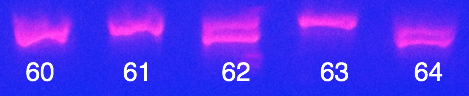
\includegraphics[width=.7\textwidth]{photo}
	\caption[Photographie d'un gel d'agarose placé sur une plaque à UV]{Photographie d'un gel d'agarose placé sur une plaque à UV. Les individus placés dans les puits 60, 61 et 63 sont des femelles car il n'y a qu'une seule bande. Les individus des puits 62 et 64 sont des mâles.}
	\label{fig:photo}
\end{figure}


\subsection{Séquences mitochondriales}

Pour chaque individu, un fragment de 682 paires de bases de la région de contrôle a été amplifié par PCR puis séquencé. Chaque mélange réactionnel de 25$\mu$L contenait : 2,5$\mu$L de tampon 10X, 2mM de MgCl$_2$, 0,25mM de dNTP, 0,125$\mu$M des amorces Dlp1.5 (5'-\textsc{tcacccaaagctgrarttcta}-3', \citealt{baker1998}) et Dlp8G (5'-\textsc{ggagtactatgtcctgtaacca}-3', \citealt{dalebout2005}), 0,5 unité de Taq polymérase et 2$\mu$L d'ADN (de moins de 1 à plus de 100 ng/$\mu$L selon les individus). Les conditions de PCR sont les suivantes : une première dénaturation de 3 minutes à 94ºC suivie de 40 cycles de 30 secondes de dénaturation à 92ºC, 45 secondes d'appariement à 51ºC et 45 secondes d'élongation à 72ºC. Une étape d'élongation finale de 7 minutes à 72ºC est également réalisée. Pour chaque individu, les brins sens et anti-sens de l'ADN ont systématiquement été séquencés (société GATC Biotech) afin de limiter les erreurs de sequençage. De la même façon, certains individus ont été séquencés plusieurs fois afin de s'assurer de la reproductibilité des résultats. Les séquences sont ensuite nettoyées (correction des erreurs de séquençage, élimination de la séquence des amorces) et alignées dans le logiciel \texttt{BioEdit}\texttrademark~\texttt{v7.2.5} \citep{hall1999}.


\subsection{Génotypes microsatellites}
Un total de 25 loci nucléaires microsatellites ont été ciblés. Ces marqueurs hypervariables sont décrits dans \citet{louis2014}. Leurs principales caractéristiques sont présentées dans l'annexe~\ref{microsats}. Afin de pouvoir comparer les résultats de la présente étude à ceux obtenus par Marie Louis \citep{louis2014}, des individus présentant des tailles d'allèles connus ont été utilisés en guise de marqueur de taille. Pour les 67 individus inclus dans ce travail ainsi que pour les individus de référence, les PCR ont été réalisées pour chacun des 25 loci dans les conditions décrites dans \citet{louis2014}. Le génotypage a été réalisé au laboratoire sur un séquenceur à plaques Li-Cor 4300 DNA Analyzer. Il s'agit d'un dispositif d'électrophorèse verticale dans un gel de polyacrylamide fin (0,2 millimètres d'épaisseur) extrêmement résolutif puisqu'il permet de visualiser des différences de tailles de fragments d'une paire de bases. Pour chaque marqueur et chaque individu, le génotype est donc enregistré sous la forme de 2 nombres rendant compte de la taille (en nombre de nucléotide) de chaque allèle présent.


\subsection{Vérification de la qualité des données}

% Le lecteur se moque de connaitre toutes les options logicielles existantes pour réaliser telle ou telle analyse. En revanche, il veut savoir concrètement ce qui a été fait et pourquoi, de façon à pouvoir reproduire les analyses. Il faut donc fournir le nom des logiciels utilisés avec leur numéro de version, la référence biblio présentant le logiciel ou la méthode utilisée, et la liste des paramètres utilisés dans le logiciel quand c'est pertinent.
À l'échelle du jeu de données complet, l'écart à l'équilibre de Hardy-Weinberg et l'absence de déséquilibre de liaison entre chaque paire de loci a été testé dans \texttt{Genepop~v4.2} \citep{rousset2008} avec les réglages suivants : démémorisation $= 1000$, nombre de chaînes $= 100$, nombre d'itérations par chaîne $= 1000$. La correction séquentielle de Bonferroni a été appliquée pour corriger l'augmentation de l'erreur de type I liée aux comparaisons multiples \citep{holm1979}.
La présence d'allèles nuls\footnote{allèle ne pouvant pas être détecté en raison de la présence de mutations empêchant son amplification par PCR.} a été testée dans \texttt{Microchecker~v2.2.3} \citep{oosterhoot2004} et la présence de potentiels duplicats parmi les individus biopsiés a été examinée en comparant les génotypes multilocus des individus dans \texttt{GenAlex~v6.5} \citep{peakall2012}. Enfin, la présence dans le jeu de données d'individus fortement apparentés (qui pourraient donc biaiser les inférences de structure de populations) a été vérifiée grâce au logiciel \texttt{MLRelate} \citep{kalinowski2006}. Lorsque des valeurs d'apparentements supérieures à 0.50 ont été détectées entre 2 individus, l'un des deux individus de la paire a été retiré du jeu de données \citep{viricel2014}.


\subsection{Inférences de la structure des populations}

Afin de réaliser des analyses ayant une portée régionale, les données générées lors de cette étude ont été analysées conjointement avec des données générées par Marie Louis lors de son doctorat \citep{phdLouis2014}, notamment celles concernant la Méditerranée et la façade Atlantique de la Péninsule Ibérique. Les inférences de structure de populations ont été réalisées sur la base de ce jeu de données étendu, uniquement avec les données microsatellites, et à l'aide de 3 méthodes de clustering distinctes.

\subsubsection*{\texttt{Structure~v2.3.4} \citep{pritchard2000}}

Grâce à un algorithme MCMC (Markov Chain Monte Carlo), le logiciel \texttt{Structure} permet (i) d'inférer le nombre de populations le plus vraisemblable (noté $K$) compte tenu des génotypes multilocus observés et (ii) de calculer, par individu, la probabilité d'appartenance à chacune des populations inférées. Concrètement, pour chaque simulation, l'utilisateur fixe une valeur pour $K$ et le logiciel fournit une valeur de vraisemblance globale (notée $LnPD$) pour le modèle testé, et les probabilités d'assignations individuelles. Puisque \texttt{Structure} repose sur un modèle Bayésien, il est important de ne pas se contenter d'une unique simulation pour chaque valeur de $K$ testé. Ainsi, pour chaque valeur de $K$ testée (entre 1 et 15 populations), 15 réplicats ont été réalisés afin de s'assurer de la convergence des simulations. Pour chaque simulation, une phase initiale de ``burnin'' de $50\,000$ pas permet de s'affranchir des conditions initiales, et la longueur des chaînes de Markov a été fixée à $150\,000$ après la phase de ``burnin''. Le modèle avec admixture mais sans ``LOCPRIOR'' (i.e. aucune prise en compte de l'origine géographique des individus) a été utilisé. Selon les préconisations de \citet{pritchard2000}, la valeur de $K$ retenue est celle pour laquelle la vraissemblance moyenne ($LnPD$) est la plus forte et pour laquelle la variance inter simulations est la plus faible.

\subsubsection*{\texttt{TESS~v2.3} \citep{durand2009}}

Ce logiciel produit des résultats similaires à ceux de \texttt{Structure} (i.e. nombre de populations $K$ le plus vraisemblable et assignation des individus aux populations inferées), mais permet en outre d'intégrer une information supplémentaire en guise de prior du modèle : la localisation géographique des individus. Le modèle considère en effet qu'indépendamment de leur génotype, deux individus collectés près l'un de l'autre ont plus de chances d'appartenir à la même population que deux individus collectés dans des localités éloignées \citep{durand2009}. Là encore, plusieurs valeurs de $K$ doivent être testées (ici, de 2 à 15) et pour chacune d'entre elles, 15 réplications ont été réalisées avec un modèle d'admixture BYM (Modèle Baysien, utilisant un piror non informatif sur les paramètres de variances de l'algorithme de Gibbs \cite{durand2009}) avec une chaine de longueur $1\,200$ et un burnin de $200$. Le choix de la valeur de $K$ la plus vraisemblable se fait en identifiant le point du graphique du DIC (Deviance Information Criterion) en fonction de $K$ pour lequel la rupture de pente est la plus forte.

La visualisation des résultats produits par \texttt{TESS} peut prendre 2 formes :
\begin{enumerate}
	\item un barplot présentant, pour chaque individu, les probabilités d'assignation à chaque populations inférées. Ce mode de visualisation est identique à celui proposé par \texttt{Structure}
	\item des cartes de probabilités (une carte par population inférée) permettant une visualisation spatiale des contours probables des populations. Ces cartes ont été produites dans le logiciel \texttt{R~v3.2.3} \citep{rct2015} grâce aux packages \texttt{fields~v8.4-1} \citep{nychka2015}, \texttt{mapdata~v2.2-6} \citep{becker2016}, \texttt{shape~v1.4.2} \citep{soetaert2014} et \texttt{marmap~v0.9.5} \citep{pante2013}.
\end{enumerate}

\subsubsection*{DAPC, \texttt{adegenet~v2.0.1} \citep{jombart2008}}

La DAPC (Analyse Discriminante sur les Composantes Principales) est une approche très différente de celles développées dans \texttt{Structure} et \texttt{TESS}. En effet, cette méthode ne fait aucune hypothèse concernant le mode d'évolution des marqueurs génétiques, le modèle d'admixture ou l'équilibre de Hardy-Weinberg. C'est une méthode d'analyse multivariée classique qui permet de visualiser les structures les plus marquantes d'un jeu de données multivariées dans un espace en dimension réduites. Ici, l'analyse tente d'identifier les combinaisons linéaires d'allèles permettant de maximiser la variance inter-cluster tout en minimisant la variabilité intra-cluster.
Implémentée dans le package \texttt{adegenet} \citep{jombart2008}, cette méthode se déroule en deux étapes.
\begin{enumerate}
	\item Dans un premier temps, la méthode des $K$-moyennes est utilisée pour tester plusieurs valeurs de $K$ (ici, de $K=1$ à 65) et plusieurs solutions de clustering sont comparées à l'aide du BIC (Bayesian Information Criterion). La valeur de $K$ la plus vraisemblable est celle pour laquelle la plus faible valeur de BIC est observée. Si aucun minima n'est visible sur la courbe du BIC en fonction de $K$, c'est alors la valeur pour laquelle une rupture de pente est observée qui doit être retenue \citep{jombart2008}.
	\item Dans un second temps, une ACP est réalisée sur les données génotypiques. Les résultats de cette ACP (i.e. les composantes principales) et des $K$-means (i.e. solution de clustering la plus vraisemblable) sont utilisées pour réaliser une analyse discriminante permettant de visualiser les résultats dans un plan portant la plus grande part de la variabilité totale du jeu de données.\\[1pc]
\end{enumerate}



\subsection{Caractérisation des populations}

Pour caractériser ces populations, des indices de diversité génétique ont été calculés pour les données microsatellites et mitochondriales.

\subsubsection*{Marqueurs microsatellites}

Pour mesurer le niveau de différenciation génétique entre populations, les $F_\textrm{ST}$ \citep[méthode de][]{weir1984} et les $\rho_\textrm{ST}$ \citep[méthode de][]{michalakis1996} ont été calculés pour chaque paire de populations dans \texttt{Genepop~v4.2} \citep{rousset2008} avec une distance minimale de 0.0001 entre les échantillons à prendre en compte pour la régression suivis de 1000 permutations pour le test de Mantel. Le $F_\textrm{ST}$ est un indice de fixation qui permet d'estimer la différenciation génétique existant entre 2 populations en terme de fréquences alléliques. Le $\rho_\textrm{ST}$ est un homologue du $F_\textrm{ST}$ qui tient compte de la taille des allèles, et donc de leurs relations phylogénétiques.

Pour chaque population et pour le jeu de données complet, les $F_\textrm{IS}$\footnote{indice de fixation mesurant l'appariement non aléatoire des allèles au sein des individus d'une population. Il rend compte du niveau de déficit en hétérozygotes (par rapport aux proportions attendues à l'équilibre de Hardy-Weinberg) dû à la consanguinité dans les populations.}, hétérozygotie observées ($H_o$) et attendues à l'équilibre de Hardy-Weinberg ($H_e$) ont été calculés dans \texttt{Genepop~v4.2} \citep{rousset2008}. Enfin, la richesse allélique ($R_{all}$) a été obtenue grâce au package \texttt{hierfstat} dans \texttt{R~v3.2.3} \citep{rct2015}. C'est un indice qui permet les comparaisons de diversités génétiques entre échantillons d'effectifs différents. Lorsque les échantillons issus de différentes populations sont de tailles différentes, les richesses alléliques sont obtenues par une méthode de raréfaction qui permet de ramener la taille de chaque échantillon à celle du plus petit échantillon, rendant ainsi les comparaisons possibles \citep{hurlbert1971}.

\subsubsection*{ADN mitochondrial}

Le package \texttt{Pegas~v0.9} \citep{paradis2010} a été utilisé dans \texttt{R~v3.2.3} \citep{rct2015} pour établir la liste des haplotypes présents dans le jeu de données, calculer leur fréquence et estimer le nombre de migrants pour chaque population selon la méthode de \citet{barton1986}. Pour visualiser les relations phylogénétiques entre les haplotypes identifiés, un réseau a été construit dans \texttt{Network~v5.0.0.0} \citep{bandelt1999} par la méthode du median-joining \citep{cassens2003}.

De la même manière que le $\rho_\textrm{ST}$ permet de calculer la différenciation génétique en tenant compte de la taille des allèles nucléaires, le calcul des $\Phi_\textrm{ST}$ par paires de populations permet d'estimer la différenciation génétique en tenant compte de la distance génétique séparant les haplotypes mitochondriaux. Les statistiques $\Phi$ ont ainsi été calculées dans \texttt{Arlequin~v3.5.2.2} \citep{excoffier2010} en utilisant le modèle de mutation $K80$ identifié comme étant le plus probable pour nos données dans \texttt{Jmodeltest~v2} \citep{santorum2014}.

Enfin, pour chaque population et pour le jeu de données complet, le nombre de sites polymorphes ($S$), la diversité nucléotidique ($\pi$) et haplotypique ($h$) \citep[selon la méthode décrite par][]{tajima1983} et l'indice $D$\footnote{Cet indice permet de mettre en évidence des effets sélectifs ou des changements de taille des populations en comparant deux estimateurs distincts de $\theta = 4\times Ne \times \mu$, l'un basé sur le nombre de sites ségrégeants $S$, l'autre basé sur la diversité nucléotidique $\pi$ (avec $Ne$, la taille efficace de la population et $\mu$, le taux de mutation).} \citep{tajima1989} ont été calculés dans \texttt{DnaSP~v5.10.1} \citep{librado2009}.


\section{Résultats}



\subsection{Qualité des données et sélection des marqueurs}

Au cours de cette étude, 67 \emph{Tursiops truncatus} méditerranéens ont été génotypés pour 25 marqueurs microsatellites (voir liste des marqueurs en annexe, table~XXX). Pour 26 individus, l'état de putréfaction avancé des tissus a conduit à des rendements d'extraction d'ADN inférieurs à 10 ng$.\mu \textrm{L}^{-1}$ (figure~\ref{fig:concentration}). Ces rendements n'ont pas permis l'amplification des marqueurs nucléaires chez ces individus. Par ailleurs, une relation parent-enfant a été identifiée pour 2 individus. L'un des 2 membres de la paire a été retiré afin d'éviter les biais lors des inférences de structure de population. Aucun duplicat de biospie n'a en revanche été détecté.
En outre, sur les 25 marqueurs génotypés, 13 ont dû être ignorés : 6 d'entre eux possédaient des niveaux de déséquilibre de liaison très significatifs ($p<0,01$), 4 présentaient un taux de données manquantes superieur à 60\% et 3 loci ont été retirés car ils n'étaient pas lisibles sur les gels. Au final, le jeu de données nucléaire comporte 12 loci et 40 individus méditerranéens. Afin de donner une dimension plus regionale aux analyses ultérieures, 81 individus analysés par Marie Louis \citep{phdLouis2014} ont également été considérés (33 issus de Galice, 39 de Cadiz et Gibraltar et 9 du Sud de la France et de Corse) portant le nombre total d'individus analysés ici à 121 pour les données nucléaires.

63 séquences mitochondriales nouvelles de 682 paires de bases ont été obtenues au cours de cette étude. Ces séquences contiennent un total de 37 sites ségrégeants définissant 32 haplotypes distincts. 75 séquences obtenues par Marie Louis ont été ajoutées à notre alignement pour les analyses ultérieures (soit un total de 138 individus analysés).

\subsection{Inférence de la structure des populations}

% \emph{J'ai refait les graphique pour leur donner une unité. Là encore, il faut travailler la cohérence globale du document. On ne parle que de la structure globale dans un premier temps et on montre que les 3 approches conduisent au même résultat : $K=3$. Ça n'est qu'ensuite que l'on présente un barplot, les cartes et la DAPC.}

L'inférence du nombre de populations le plus vraisemblable dans notre jeu de données a été obtenu par trois méthodes distinctes. Les résultats obtenus grâce au logiciel \texttt{Structure} \citep{pritchard2000} indiquent que le nombre de populations le plus vraissemblable compte tenu des seules données nucléaires est $K=3$ (figure~\ref{fig:lnpd}). Le même résultat a été obtenu avec le logiciel \texttt{TESS} \citep[][figure~\ref{fig:dic}]{durand2009} qui, outre les informations génétiques, prend également en compte les coordonnées géographiques de chaque individu. 
Enfin, l'Analyse Discriminante sur les Composantes Principales, qui n'est pas influencée par la nature génétique des données (e.g. la DAPC ne fait pas d'hypothèse concernant le modèle de mutation des marqueurs utilisé, ou ne cherche pas à identifier des populations à l'équilibre de Hardy-Weinberg, \citealp{jombart2008}) arrive au même résultat (figure~\ref{fig:bic}).

\begin{figure}[htpb]

{\centering 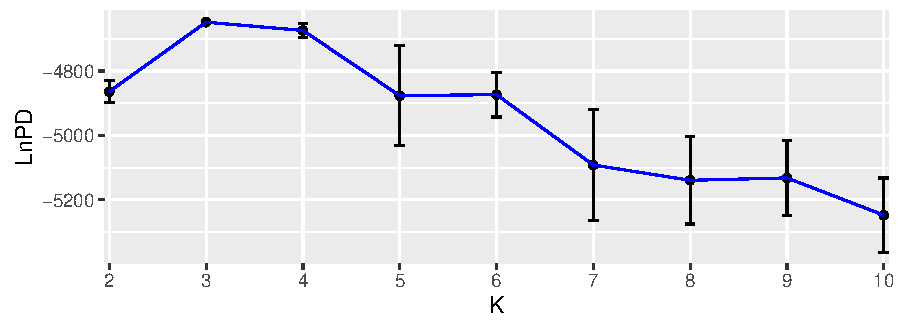
\includegraphics[width=\maxwidth]{figure/lnpd-1} 

}

\caption[Vraisemblance ($LnPD$) en fonction de $K$.]{Vraisemblance ($LnPD$) en fonction de $K$. Les points correspondent aux moyennes de 15 simulations et les barres d'erreurs représentent les écart-types. Le nombre de populations $K$ le plus vraisemblable est celui qui présente une valeur moyenne maximale et un écart-type le plus faible \citep{pritchard2000}.}\label{fig:lnpd}
\end{figure}



\begin{figure}[htpb]

{\centering 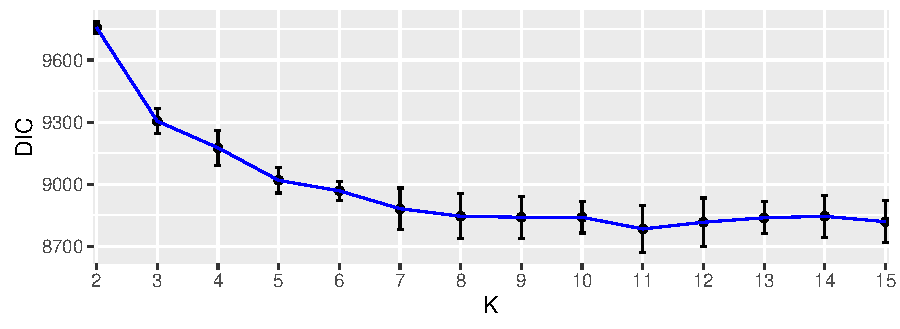
\includegraphics[width=\maxwidth]{figure/dic-1} 

}

\caption[Deviance Information Criterion (DIC) en fonction de $K$.]{Deviance Information Criterion (DIC) en fonction de $K$. Les points correspondent aux moyennes de 15 simulations et les barres d'erreurs représentent les écart-types. Le nombre de populations $K$ le plus vraisemblable est celui pour lequel la rupture de pente la plus forte est observée \citep{durand2009}.}\label{fig:dic}
\end{figure}




\begin{figure}[htpb]

{\centering 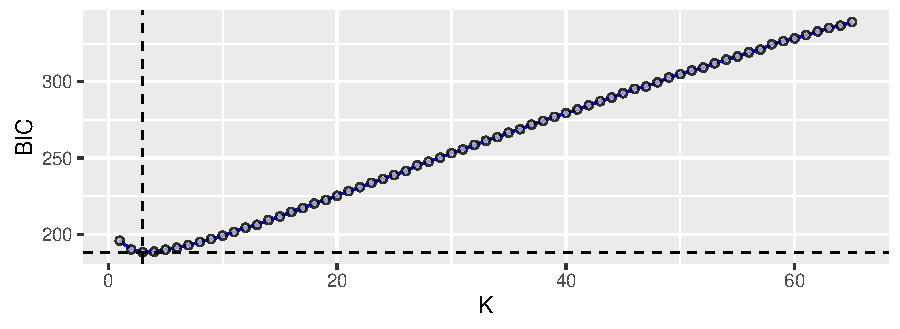
\includegraphics[width=\maxwidth]{figure/bic-1} 

}

\caption[Bayesian Information Criterion (BIC) en fonction de $K$.]{Bayesian Information Criterion (BIC) en fonction de $K$. Le nombre de populations $K$ le plus vraisemblable est celui pour lequel la valeur de BIC est minimale \citep{jombart2008}.}\label{fig:bic}
\end{figure}



Les résultats d'assignation des individus aux 3 populations inférées par les différents logiciels, sont très proches. Seuls les probabilités d'assignation calculées par \texttt{TESS} sont présentées ici (figure~\ref{fig:barplot}) puisque ces mêmes résultats ont été utilisés pour réaliser des cartes de probabilité d'appartenance à chacune des 3 populations inférées (voir figure~\ref{fig:probamap}).

\begin{figure}[htpb]

{\centering 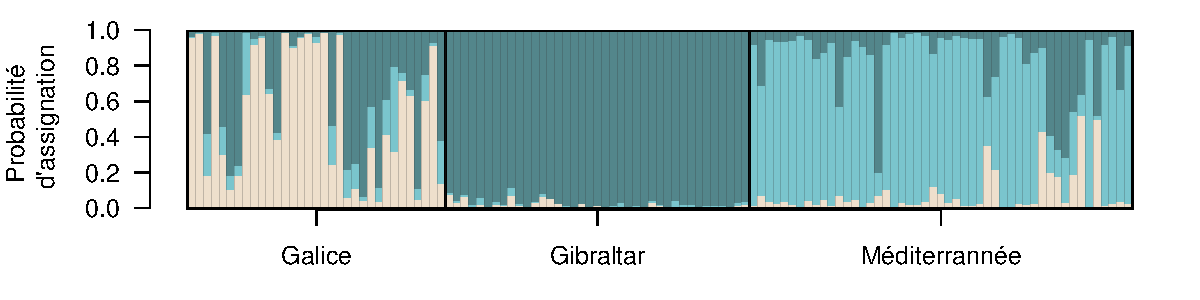
\includegraphics[width=\maxwidth]{figure/barplot-1} 

}

\caption[Probabilités d'assignations individuelles à chaque population inférée par TESS]{Probabilités d'assignations individuelles à chaque population inférée par TESS. Les individus ont été classés par longitude croissante et les zones géographiques d'origine sont indiquées. Chaque couleur correspond à l'une des 3 populations inférées.}\label{fig:barplot}
\end{figure}



Les assignations d'individus à chacune des 3 populations inférées sont globalement cohérentes avec la localisation géographique d'où sont issus les individus. En effet, 82\% des individus sont assignés à la population dont ils sont issus (58\% pour les individus de Galice, 100\% pour les individus issus de Cadiz et du Détroit de Gibraltar et  84\% des individus de Méditerranée, voir figure~\ref{fig:barplot} et table~\ref{table:assignation}). Toutefois, près de 40\% des individus échantillonnés en Galice ont une forte probabilité d'assignation à la population de Gibraltar (i.e. 13 individus sur 33, table~\ref{table:assignation}).

\begin{table}[ht]
\centering
\caption[Assignation des individus aux 3 populations inférées.]{Assignation des individus aux 3 populations inférées. Les 3 régions d'origine sont indiquées en ligne et les populations inférées en colonne. Ainsi, sur les 33 individus issus de Galice, 19 sont assignés à cette même population, 13 sont assignés à la population de Gibraltar, et 1 à la population méditerranéenne.}
\label{table:assignation}
\begin{tabular}{rrrr}
  \toprule
 & Galice & Gibraltar & Méditerranée \\ 
  \midrule
Galice &  19 &  13 &   1 \\ 
  Gibraltar &   0 &  39 &   0 \\ 
  Méditerrannée &   2 &   6 &  41 \\ 
   \bottomrule
\end{tabular}
\end{table}

Les cartes de probabilité délimitant les contours probables des populations reflètent bien ce résultat (figure~\ref{fig:probamap}). En effet, seuls les individus du Sud de la Galice semblent former une population distincte. Les individus du Nord de la Galice sont en revanche associés aux individus échantillonnés autour du Détroit de Gibraltar et à quelques individus du Sud de la Corse. Enfin, les individus génotypés ors de cette étude forment une population méditerranéenne distincte.

\begin{figure}[htbp]
	\centering
		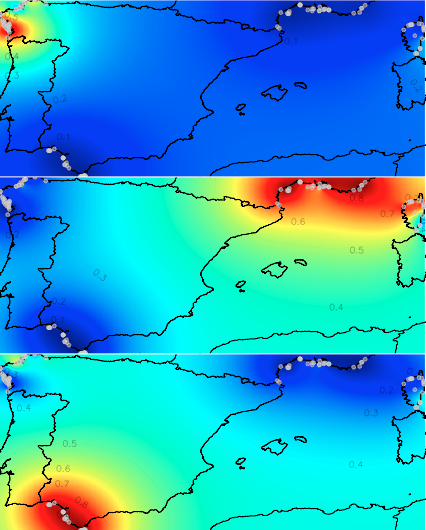
\includegraphics[width=.9\textwidth]{map_clusters_3}
	\caption[Cartes de probabilité d'appartenance aux populations inférées.]{Cartes de probabilité d'appartenance à chacune des 3 populations inférées. Chaque carte présente les probabilité d'appartenir à l'une des 3 populations inférées. Les probabilités augmentent en passant du bleu (probabilité nulle d'appartenir à la population) au rouge (probabilité maximale d'appartenir à la population).}
	\label{fig:probamap}
\end{figure}

Enfin, les regroupements produits par la DAPC sont tout à fait cohérents avec les résultats de \texttt{TESS} et \texttt{Structure} (voir figure~\ref{fig:DAPC}). Trois groupes sont clairement identifiés et correspondent aux mêmes populations que celle identifiées par les autres méthodes. Seuls 0.2\% des 121 individus ne sont pas assignés aux mêmes populations que précédemment.

\begin{figure}[htbp]
	\centering
		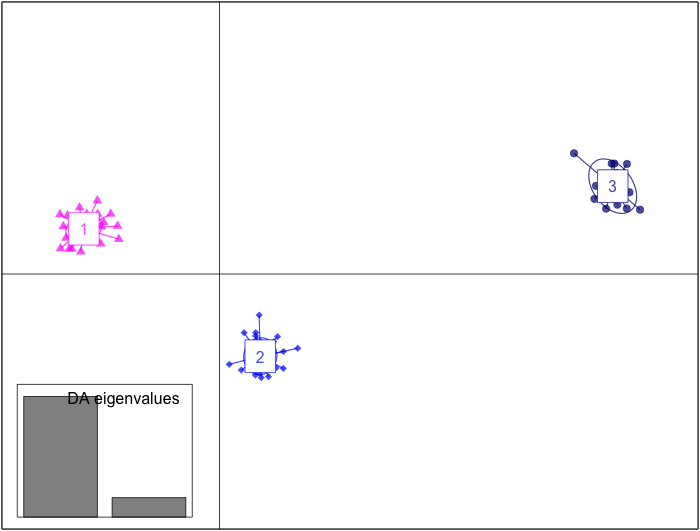
\includegraphics[width=.7\textwidth]{DAPC}
	\caption[DAPC]{La DAPC présente bien les trois clusters distinctement. Le cluster 1 (rose) correspond à la population des individus de la Méditerranée Nord Occidentale (MNO), le cluster 2 (bleu) à la population des individus de Gibraltar et le cluster 3 (violet) à la population des individus de Galice. Le graphique des ``DA eigenvalues'' correspond au pourcentage d'information porté par les axes. L'axe un (horizontal) porte environ 90 pour-cent d'information, et l'axe deux (vertical) en porte environ 10. Les composantes principales sont elles mêmes des combinaisons linéaires des variables de départ, c'est à dire des loci. Les individus proches sont alors ceux qui ont des allèles comparables.}
	\label{fig:DAPC}
\end{figure}


Afin d'affiner les résultats précédents et dans l'optique de mettre en évidence une éventuelle structure de population hiérarchique, la même approche que précédemment a été mise en \oe uvre, mais uniquement pour les individus assignés à la population méditerranéenne. Ces analysent ne concernent donc quasiement que les individus génotypés lors de cette étude (individus de Méditerranée Nord Occidentale).

\begin{figure}[htpb]

{\centering 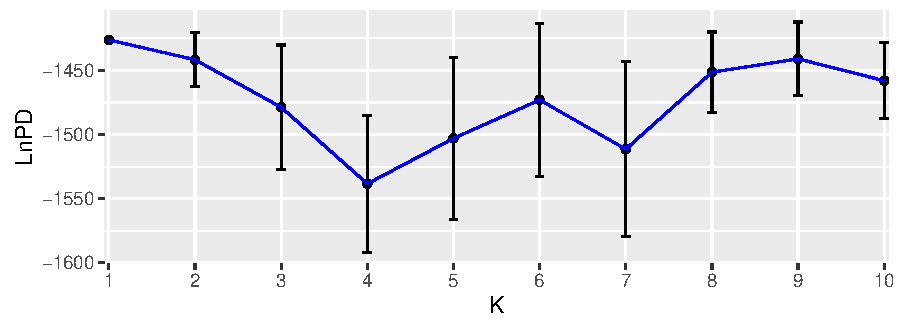
\includegraphics[width=\maxwidth]{figure/lnpd2-1} 

}

\caption[Vraisemblance ($LnPD$) en fonction de $K$.]{Vraisemblance ($LnPD$) en fonction de $K$. Les points correspondent aux moyennes de 15 simulations et les barres d'erreurs représentent les écart-types. Le nombre de populations $K$ le plus vraisemblable est celui qui présente une valeur moyenne maximale et un écart-type le plus faible \citep{pritchard2000}.}\label{fig:lnpd2}
\end{figure}



L'examen des résultats produits par \texttt{Structure} (figure~\ref{fig:lnpd2}) montre qu'une unique population méditerranéenne semble être la plus probale. En effet, le $LnPD$ moyen le plus fort est observé pour $K=1$, de même pour l'écart-type le plus faible. Ce même résultat a été obtenu avec la DAPC qui montre un BIC le plus faible pour $K=1$ (BIC = 179). Enfin, \texttt{TESS} ne permet pas de tester l'hypothèse $K=1$, ce logiciel n'a donc pas été utilisé ici.

\subsection{Caractérisation des populations}

\begin{table}[htpb]
\begin{center}
\begin{minipage}{.48\textwidth}
\centering
\caption{$F_\textrm{ST}$ par paire de populations}
\label{table:fst}
\begin{tabular}{rrr}
\toprule
   &   Galice   &    Gibraltar    \\
\midrule
Gibraltar   &   0.104 (*) 	& - \\
Méditerranée   &   0.139 & 0.055 (**) \\
\bottomrule
\end{tabular}

\end{minipage}
\hfill
\begin{minipage}{.48\textwidth}
\centering
\caption{$\rho_\textrm{ST}$ par paire de populations}
\label{table:rho}
\begin{tabular}{rrr}
\toprule
   &   Galice   &    Gibraltar    \\
\midrule
Gibraltar   &   0.070 (**) 	& - \\
Méditerranée   &   0.266 (*) & 0.151 \\
\bottomrule
\end{tabular}

\end{minipage}
(*)=significatif à 0.05; (**) = significatif à 0.01; (***) = significatif à 0.001
\end{center}
\end{table}

Les $F_\textrm{ST}$ par paires de population sont globalement faibles et comparables à ceux calculés par Marie Louis (REF). La différenciation la plus forte est observée entre les populations de Méditerranée et de Galice (0.1390, table~\ref{table:fst}). Elle est presque 3 fois plus forte qu'entre les populations de Gibraltar et de Méditerranée.

Comme pour les $F_\textrm{ST}$, le $\rho_\textrm{ST}$ (qui tient compte des distances génétiques entre les allèles des populations comparées) le plus fort est observé entre les populations de Méditerranée et de Galice. En revanche, la valeur la plus faible est cette fois observée entre les populations de Gibraltar et de Galice (table~\ref{table:rho}).

\begin{table}[htpb]
\centering
\caption[Indices synthétiques pour les marqueurs microsatellites.\label{micro}]{Indices synthétiques pour les marqueurs microsatellites. $N$ : nombre d'individus, $F_\textrm{IS}$ : coefficient de consanguinité, $Ho$ : hétérozygotie observée, $He$ : hétérozygotie attendue, $R_{All}$ : Richesse allélique.}
\label{micro}
\begin{tabular}{rrrcrrr}
\toprule
 & $N$ & $F_\textrm{IS}$ & P value $F_\textrm{IS}$  & $Ho$ & $He$ & $R_{All}$ \\
\hline
Galice 			&	21	&	0.1433	& 0.092 &	0.6332	&	0.7391	&	6 \\
Gibraltar 		&	58	&	0.0297	& 0.023 &	0.7471	&	0.7700	&	7.6205\\
Méditerranée 	&	42	&	-0.0120	& 0.009 &	0.7929	&	0.7766	&	8.1162 \\
\midrule
Global 			&	121	&	0.1610	& 0.41 &	0.7933	&	0.7791	&	11.4166 \\
\bottomrule
\end{tabular}
\end{table}

La table \ref{micro} présente les différents indices servant à comparer la diversité génétique des populations à l'aide des données microsatellites avec d'autres études. Le $F_\textrm{IS}$ est un indice qui renseigne sur les taux de consanguinité. Ce taux est le plus fort dans la population de Galice comparé aux autres populations. Les hétérozygoties attendues et observés (Ho) ont servis pour le calcul des Fis. La richesse allélique $R_{All}$ donne une idée de la diversité réelle des populations, et donc de leur taille. Ici la $R_{All}$ est relativement similaire entre les populations.

\begin{table}[!]
\centering
\caption[Table des indices génétiques pour les ADN mitochondriaux \label{mito}]{$N$: Nombre d'individus; $NH$: Nombre d'haplotype; $S$: Nombre de sites polymorphiques; $h$: Diversité haplotypique $Pi$: Diversité nucléotidique, $D Taj$: D de Tajima}
\label{mito}
\begin{tabular}{rrrrrrr}
\toprule
 & $N$	&	$NH$	&	$S$	&	$h$	&	$Pi$	& $D Taj$\\
\hline
Galice &	18	&	6	&	16	&	0.562	&	0.0064 & -0.1916	\\
Gibraltar &	52	&	18	&	30	&	0.918	&	0.01295 & 0.9547	\\
Méditerranée &	39	&	12	&	28	&	0.808	&	0.0110	& 0.3372 \\
Non assigné	&	29	&	13	&	30	&	0.736	&	0.0091	& -0.79244	\\
\midrule
Global &	138	&	32	&	37	&	0.0.906	&	0.01285 & 0.7109	\\
\bottomrule
\end{tabular}
\end{table}

La table \ref{mito} présente les différents indices servant à comparer la diversité génétique des populations à l'aide des données mitochondriales avec d'autres études. Le nombre d'haplotype donne une idée de la diversité de la population. Le nombre de sites polymorphes est deux fois inférieur en Galice par rapport aux autres populations. La diversité haplotypique et nucléotidique sont aussi les plus basses pour la population de Galice par rapport aux autres populations. Le D de Tajima est aussi un indice de différenciation. Plus les valeurs sont proches de zéro, plus les individus auront des allèles en commun; plus elles sont proches de un, moins les individus auront des allèles en commun. La population de Gibraltar présente beaucoup d'allèles en commun (0.9547), les autres populations ne présentent pas beaucoup d'allèles en commun (bien que de D de Tajima pour la Méditerranée est de 0.3372). Le D de Tajima global est néanmoins assez fort (0.7199).

Le taux de migrants entre population a aussi était calculé, avec 2.605 migrants par génération entre les populations. La moyenne des fréquences allèles privée est de 0.0477864. Un allèle privé et un allèle qui n'existe que dans une seule population, si il y a beaucoup de migrants, il y aura moins d'allèles privés.

\begin{figure}[h]
   \centering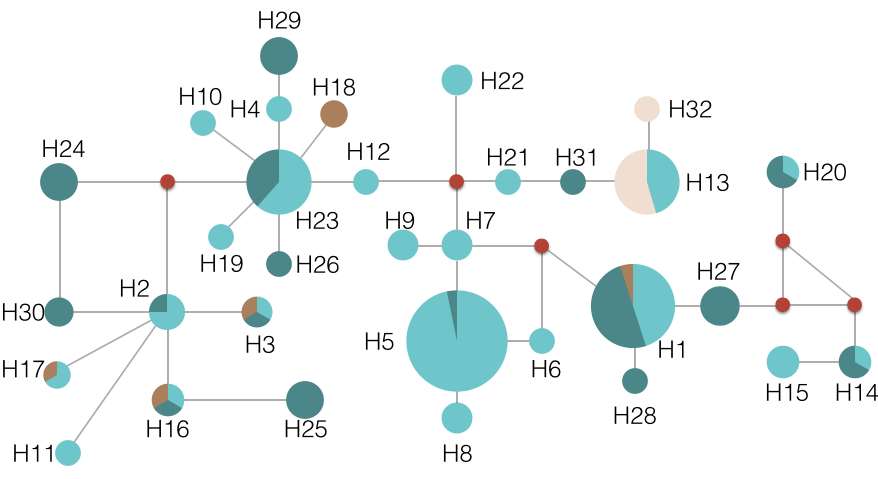
\includegraphics[scale=0.4]{reseau}
   \caption[Réseau d'haplotypes.]{Réseau des 32 haplotypes. Les disques rouges représentent les vecteurs médians. Les diagrammes représentent la proportion d'individus par population (marron pour l'Itlaie, beige pour la Galice, bleu clair pour la Méditerranée et bleu foncé pour Gibraltar)}
\end{figure}
\FloatBarrier

Pour ce réseau, basé sur les données mitochondriales, cinq individus provenant d'Italie ont été volontairement coloriés (en marron). Ces individus non pas pu être exploités pour les données microsatellites.
Ce réseau de 32 haplotypes (réalisé à partir des données placées sous Network) démontre que la population de Galice (Haplotypes 13 et 32) est relativement à part. Les individus italiens sont relativement bien répartis dans ce réseau, comme les deux autres populations (de MNO et de Gibraltar). Ce qui démontrent un échange d'individus entre ces trois populations, mais un échange faible avec la population galicienne.

\section{Discussion} 

Les résultats de cette étude ont révélé différents degrés de différenciation génétique dans la zone d'étude de la Méditerranée étendue à la Galice. Un schéma global de structuration de la population a été détectée par DAPC et les cartes de krigeage, et, dans une moindre mesure, par une approche de classification bayésienne. Les données d'ADN mitochondrial et microsatellites ont révélé une plus forte divergence entre les sites d'échantillonnage géographiquement éloignés (e.g. Galice et Méditerranée Nord Occidentale (MNO)).

Les grands dauphins échantillonnés lors de cette étude et les individus méditerranéens collectés par Marie Louis seraient répartis en trois populations dans la Méditerranée étendue à la Galice: 

Une population galicienne, présentant majoritairement des individus autochtones à cette région, exception faite pour deux individus appartenant à cette population retrouvés en MNO. 

Une population en MNO, dans laquelle on ne retrouve qu'uniquement des individus de ce milieu ci. Aucun autre individu rattaché à une autre population n'y a été échantillonnés. 

Et enfin une population provenant de Gibraltar, qui présente essentiellement des individus échantillonnés en Andalousie, mais aussi des individus retrouvés en Galice et en MNO. 

Les cartes de krigeage ont montrées que des individus du sud de la Corse sont rattachés à la population de Gibraltar. L'étude de la sous-structure de population en MNO n'a pourtant démontrée la présence que d'une seule population dans cette région. Les individus provenant d'Italie n'ont pas pu être intégrés aux données microsatellites, ainsi il n'a pas était possible d'établir si ils faisaient partis uniquement de l'ensemble de MNO, ou au contraire, si ils se serraient rattachés à ces individus du sud de la Corse, et peut-être démontré la présence d'une sous-population. Néanmoins, les données des individus italiens ont pu être utilisés via l'ADN mitochondrial. Celles-ci ont démontré avec le réseau d'haplotypes que les individus italiens présentent des haplotypes partagés avec l'ensemble des populations de MNO et de Gibraltar. Les individus italiens seraient alors bien intégrés à l'ensemble d'une seule et même population en MNO, du fait des haplotypes échangés, et donc d'échanges d'individus. Un échantillonnage plus intense, et couvrant une zone plus large permettrait concrètement de lever le doute sur la présence d'une sous-population avec des individus du sud de la Corse. \citet{carnabuci2016} ont réalisé une étude des réseaux de \emph{Tursiops truncatus} dans le sanctuaire Pelagos à partir de données de photo-identifications. Il semblerait qu'il y ait cinq groupes vivant dans ce sanctuaire. Un groupe Alpha vivant au Nord de la Méditerranée le long des côtes italiennes, un groupe Beta vivant au nord ouest de la corse, un groupe Epsilon vivant dans le sud de la France et au nord est de la Corse, un groupe Delta vivant dans l'archipel toscan, et enfin un groupe Gamma vivant au sud de la Corse. Ce groupe Gamma pourrait être celui des individus retrouvés au sud de la Corse dans notre étude et qui ne faisaient pas parti du cluster MNO selon les cartes de krigeage.

\citet{natoli2005habitat} ont aussi utilisé des microsatellites pour différencier les différentes populations des \emph{Tursiops} sur certaines régions de Méditerranée, et ils ont trouvé une divergence entre les populations de la Mer Tyrrhénienne et d'Espagne. Cependant, des individus de la Mer Tyrrhénienne appartenaient à la population de la Mer Adriatique. Nos individus italiens ayant été échantillonnés en Mer Tyrrhénienne mais semblant faire parti de la population de MNO, il se pourrait qu'il y ait une population plus large regroupant la MNO, la Mer Tyrrhénienne et la Mer Adriatique. Néanmoins, les individus du sud de la Corse sèment le doute. Soit ils font partis d'une petite population, soit ils s'inscrivent dans un sous ensemble bien plus grand mais non échantillonnés (e.g. Sardaigne, côtes de l'Afrique du Nord..). Il faudrait pouvoir acquérir des données microsatellites pour des individus d'Italie et plus d'individus du sud de la Corse afin de pouvoir trancher.

Les individus de la Mer Méditerranée ont été considérés comme vivant dans des zones côtières dans les études précédentes \citep{natoli2004population, natoli2005habitat}, ce qui contraste avec le niveau élevé de diversité génétique trouvé dans cette étude et qui indiquent des populations pélagiques. Selon \citet{gnone2011distribution}, certains groupes côtiers seraient résidents mais des mouvements ont été signalés entre la Corse et la France, ce qui indique que les individus ont traversé les eaux pélagiques. De plus, l'utilisation de l'habitat pélagique a été confirmée par des relevés aériens menés pendant l'hiver 2011/2012 où les dauphins étaient principalement vus en eau profonde ($> 200$ mètres) \citep{louis2014}.

Le réseau d'haplotypes présente les individus galiciens comme étant en marge des autres populations, car les deux haplotypes présents (H13 et H32) sont en bout de branche du réseau, ce qui pourrait signifier une divergence évolutive. De plus, la population galicienne présente un nombre de sites polymorphiques deux fois moins important que les deux autres populations (16 sites polymorphes pour la Galice, contre 30 pour Gibraltar et 28 pour la MNO), ce qui pourrait signifier un brassage génétique avec des individus proches. En outre, les indices de diversité haplotypiques et nucléotidiques sont les plus faibles pour cette population, ce qui démontre une population avec une faible diversité génétique, donc avec peu d'échanges inter-populationnels. Un équilibre mutation/dérive génétique se fait au sein des populations, et est mesuré par cet indice de diversité nucléotidique. Cet indice est le facteur du taux de mutation et de la taille de population par quatre. Le taux de mutation est ici plus faible que les autres populations (nombre de sites polymorphiques) mais la taille de cette population est aussi bien plus faible que les deux autres (18 contre 52 et 39 individus). Ceci pourrait expliquer ce faible taux de diversité. Le D de Tajima est quant à lui très faible (même négatif) pour la population galicienne, ce qui démontre que les individus ont beaucoup d'allèles en commun. De plus, le $F_\textrm{IS}$ calculé avec les données microsatellites pour la population galicienne prouve un taux de consanguinité certes faible ($0.1433$, pvalue: $0.092$), et comparable avec des valeurs similaires dans la littérature \citep{louis2014, phdLouis2014}, mais qui est de loin le plus fort en comparaison avec les autres populations (sept fois plus important que Gibraltar, et 14 fois plus que la MNO). La population galicienne serait donc bien en marge des autres populations et présenterait peu d'échanges avec les autres populations. Cependant, des individus échantillonnés en Galice appartiennent à la population de Gibraltar. L'explication de ce cas pourrait être apporté par le fait que la Galice présenterai deux populations selon \citet{louis2014}. Une population serait pélagique et une autre côtière. \citet{lowther2014} présentent des indices de diversités nucléotidiques ($Pi$ = $0.005$) similaires pour leurs individus côtiers comparés aux individus Galiciens ($Pi$ = $0.006$), et des indices de diversités nucléotidiques similaires pour leurs individus pélagiques ($Pi$ = $0.022$) comparés aux individus de Gibraltar ($Pi$ = $0.012$) et de MNO ($Pi$ = $0.011$) de notre étude. De plus, dans leur étude, \citet{lowther2014} présentent aussi des richesses alléliques supérieures pour les populations pélagiques, et inférieures pour les populations côtières. La population de notre étude présentant la richesse allélique la plus faible est la population de Galice ($6$, contre $7.6205$ pour Gibraltar et $8.1162$ pour la MNO). La population côtière pourrait être celle qui échange peu d'individus avec les autres populations, ce qui expliquerait les faibles taux des indices de diversité trouvé dans la population galicienne. Les individus pélagiques pourraient donc former une population à part entière, et du fait de leur pélagicité rencontrer différentes populations comme celles de Gibraltar. En d'autres termes, des individus de la population pélagique de Gibraltar pourraient se mélanger occasionnellement à la population pélagique galicienne. La population pélagique galicienne et la population côtière galicienne n'aurait pas ou peu d'échanges d'individus selon \citet{louis2014}. \citep{duffield1983hematology} ont comparé l'hématocrite\footnote{ Pourcentage relatif du volume des cellules circulant dans le sang par rapport au volume total du sang} de populations côtières et pélagiques de \emph{Tursiops} de Floride. Les dauphins du large présentent des valeurs d'hématocrite plus fortes par rapport aux côtiers. Des croisements en captivité de dauphins des deux écotypes ont produits des animaux avec des profils hématologiques intermédiaires, ce qui indique que des facteurs génétiques sont en grande partie responsables des différences entre les deux écotypes. Des populations de grands dauphins vivant sur une même zone géographique mais avec deux comportements différents peuvent donc bien être séparés génétiquement. Cette différence de niche écologique pourrait s'être orchestré selon une préférence alimentaire. Mais selon l'étude de \citet{gaspari2015population}, l'analyse des isotopes stables des individus dans l'Adriatique centrale montre que les grands dauphins changent facilement de proie, dépendant probablement de la disponibilité des proies \citep{holcer2012ecology}.

Cependant l'effet saisonnier ne pas être estimé avec les méthodes génétiques. Il se peut que des individus, voir des populations, changent de milieu au cours des saisons. En effet, cela serait le cas de populations de \emph{Tursiops} en MNO selon \citep{Laran2016}. Leur modélisation montre le passage d'une distribution clairement côtière en été, à une répartition plus pélagique pendant l'hiver, à l'exception de l'archipel toscan, où les grands dauphins sont présents dans les deux saisons.

Il se pourrait que les \emph{Tursiops} est une structure génétique populationnelle à une petite échelle géographique. Ceci a été suggéré par \citet{krutzen2004population} à Shark Bay, en Australie , par \citet{sellas2005mitochondrial} dans l'Atlantique Nord-Ouest (au Mexique), et plus récemment par \citet{ansmann2012dolphins} pour les grands dauphins côtiers (\emph{Tursiops aduncus}) à Moreton Bay, en Australie. Ces études et nos données impliquent la possibilité d'un modèle globale d'une différenciation à petite échelle pour ce genre.

Selon \citet{gaspari2015population}, lorsque l'on considère les écarts entre l'ADN nucléaire et mitochondrial les données peuvent être influencées par les flux de gènes sexuels. En effet, la dispersion différentielle des mâles et des femelles peut avoir une influence majeure sur la distribution des gènes maternels et bi-parentataux hérités des populations de grands dauphins \citep{hoelzel1998genetic}. Dans certaines populations, les dauphins mâles se dispersent plus souvent et plus loin que les femelles (\citep{krutzen2004population, moller2004genetic}. Alors que dans d'autres populations, il n'y a pas de différences significatives dans la dispersion entre les sexes \citep{natoli2005habitat}. Dans l'étude de \citet{gaspari2015population} sur les \emph{Tursiops} en Mer Tyrrhénienne et Adriatique, contrairement aux données d'ADN nucléaire, les séquences d'ADN mitochondrial ne montraient aucune différence entre les sites d'échantillonnages, ce qui suggère que les grands dauphins femelles peuvent avoir un rôle important dans la médiation de flux de gènes à travers le bassin. Voilà pourquoi il serait intéressant de pouvoir coupler les données du sexage obtenues lors de cette étude avec les données microsatellites et mitochondriales afin de connaitre la dispersion différentielle en fonction du sexe.

Il faut néanmoins garder à l'esprit que la majorité des individus échantillonnés provient de cétacés échoués, et parfois en état de putréfaction. Il peut alors s'écouler quelques jours, voir quelques semaines avant que le mammifère marin ne vienne s'échouer sur une côte (communication personnelle; Fabien Demaret\footnote{Observatoire PELAGIS - UMS 3462, Université de La Rochelle / CNRS - 5 allée de l’Océan - 17 000 La Rochelle}). Son lieu de découverte ne correspond pas à son lieu de mort, et donc de vie. Aucun modèle de courantologie en Mer Méditerranée n'a pu être couplé à cette étude, ne permettant donc pas d'interpoler le véritable lieu de vie des individus trouvés échoués. Il se peut alors que l'appartenance à une zone géographique d'individus soit biaisé par ce critère qui n'a pu être étudié.

Ces résultats permettent d'apporter de nouvelles informations sur la distribution et la structuration de cette espèce de cétacé en Mer Méditerranée. Les informations de cette étude aideront donc à la prise de décisions politiques pour la protection de cette espèce dans les plans de gestion des aires marines protégées de la Mer Méditerranée, et par conséquent, sur les écosystèmes englobés dans leurs habitats.


\newpage
	\begin{otherlanguage}{english}
		\singlespacing
		\begin{multicols}{2}[]
		\putbib [Bibliographie]
	\end{multicols}
\end{otherlanguage}

\end {bibunit}


\newpage
\section{Annexes}

\begin {bibunit} [newbst]

\begin{table}[h]
\centering
\caption{Table des individus par population}
\label{indpop}
\begin{tabular}{|l|lll|ll|}
\hline
Galice & \multicolumn{3}{|c|}{Gibraltar} & \multicolumn{2}{|c|}{Méditerranée} \\
\hline
G10    & C1        & C30       & G23       & G17          & ttr\_39      \\
G12    & C10       & C32       & G26       & M12          & ttr\_40      \\
G13    & C11       & C33       & G27       & M2           & ttr\_41      \\
G14    & C12       & C34       & G28       & ttr\_01      & ttr\_42      \\
G15    & C13       & C35       & G34       & ttr\_02      & ttr\_43      \\
G16    & C15       & C36       & G4        & ttr\_04      & ttr\_45      \\
G18    & C16       & C37       & G5        & ttr\_07      & ttr\_46      \\
G2     & C17       & C38       & G6        & ttr\_09      & ttr\_47      \\
G21    & C18       & C39       & G7        & ttr\_11      & ttr\_49      \\
G22    & C19       & C4        & G9        & ttr\_12      & ttr\_51      \\
G24    & C2        & C40       & M1        & ttr\_13      & ttr\_52      \\
G25    & C20       & C41       & M11       & ttr\_15      & ttr\_53      \\
G29    & C21       & C42       & M14       & ttr\_17      & ttr\_54      \\
G3     & C22       & C5        & M15       & ttr\_18      & ttr\_55      \\
G30    & C23       & C6        & M16       & ttr\_23      & ttr\_56      \\
G31    & C24       & C7        & ttr\_44   & ttr\_25      & ttr\_59      \\
G32    & C25       & C8        &           & ttr\_27      & ttr\_60      \\
G33    & C26       & C9        &           & ttr\_28      & ttr\_61      \\
G8     & C27       & G1        &           & ttr\_33      & ttr\_62      \\
M3     & C28       & G11       &           & ttr\_34      & ttr\_63      \\
M8     & C3        & G20       &           & ttr\_38      & ttr\_68      \\
\hline
Total:21 & \multicolumn{3}{|c|}{Total:58} & \multicolumn{2}{|c|}{Total:42} \\
\hline
\end{tabular}
\end{table}
\FloatBarrier

La table \ref{indpop} présente l'assignation des individus à leur population selon l'inférence réalisé à l'aide des logiciels \texttt{Structure}, \citet{pritchard2000inference}, et \texttt{TESS}, \citet{franccois2010spatially}. Les individus commençant par ttr\_ correspondent à ceux échantillonnés pour cette étude, les autres proviennent de la base de données construite et utilisé par Marie Louis lors de sa thèse \citep{phdLouis2014}.


\begin{figure}
 \begin{tiny}
\rotatebox{90}{
 \begin{tabular}{ p{2cm} p{3cm} p{5cm} p{4cm} p{2cm} p{2cm} p{1.5cm} p{1cm}p{1cm}}
 	\centering
 Marqueurs & \centering	Référence & \centering Primers 5'-3' (R et F) & \centering Motif & \centering Taille des allèles & \centering Concentrations des primers (Tous ou R/F/F* or R/F*) en µM & \centering T° annealing en °C & \centering Longueur d'onde & \centering Supprimé \tabularnewline
 EV37 & \centering \citep{valsecchi1996microsatellite} - \citep{vollmer2012developing} & \centering AGCTTGATTTGGAAGTCATGA GTTTTAGTAGAGCCGTGATAAAGTGC  & \centering (AC)24	& \centering 196-250 & \centering 0.24	& \centering 55	& \centering 800 & \centering Oui \tabularnewline
 KMW12a & \centering \citep{hoelzel1998genetic} & \centering CCATACAATCCAGCAGTC CACTGCAGAATGATGACC	& \centering (CA)n & \centering 144-168	& \centering 0.125/0.075/0.05 & \centering 46 & \centering 800  & \centering Non \tabularnewline
 MK5 & \centering \citep{krutzen2001characterization} - \citep{vollmer2012developing}& \centering CTCAGAGGGAAATGAGGCTG GTTTTGTCTAGAGGTCAAAGCCTTCC & \centering (TG)13CT(TG)2CA(TG)2(TA)2(TG)4 & \centering	205-243 & \centering 0.2 & \centering 55 & \centering 700 & \centering Oui \tabularnewline
 MK6 & \centering \citep{krutzen2001characterization} - \citep{vollmer2012developing} & \centering GTCCTCTTTCCAGGTGTAGCC GCCCACTAAGTATGTTGCAGC & \centering (GT)17 & \centering 145-191 & \centering 0.2 & \centering	55 & \centering	700 & \centering Non \tabularnewline
 MK8 & \centering \citep{krutzen2001characterization} - \citep{vollmer2012developing} & \centering TCCTGGAGCATCTTATAGTGGC GTTTCTCTTTGACATGCCCTCACC	& \centering (CA)23	& \centering 87-117	& \centering 0.2 & \centering	55	& \centering 800 & \centering Oui \tabularnewline
 MK9 & \centering \citep{krutzen2001characterization} -\citep{vollmer2012developing} & \centering CATAACAAAGTGGGATGACTCC GTTTTTATCCTGTTGGCTGCAGTG & \centering (CA)17 & \centering 166-182 & \centering 0.4 & \centering 55 & \centering 800 & \centering Oui \tabularnewline
 Tur4-87 & \centering \citep{nater2009new}	& \centering CCCCATATGATGCCTTTGTAAGTCC AATTCCTTGTAACAAACCTCTTTATCT	& \centering (GATA)8 & \centering 182-202 & \centering 0.225/0.225	& \centering 61	& \centering 800  & \centering Oui \tabularnewline
 Tur4-98 & \centering \citep{nater2009new}	& \centering GTCCCCAGAACTTAGCACACTGTC CAACTGGGGTCCAAAGAAAGAAG & \centering (GATG)10 & \centering 172-204 & \centering 0.225/0.225 & \centering 63 & \centering 800 & \centering Oui \tabularnewline
 Tur4-128 & \centering \citep{nater2009new} & \centering ACGTGCGCATGTCTTTGTCTTAT CTTTGGACGGGGAGTAGAACCTA & \centering	(GATA)11 & \centering 280-304 & \centering 0.225/0.225	& \centering 62	& \centering 800 & \centering Oui \tabularnewline
 Tur4-142 & \centering \citep{nater2009new} & \centering GGCCCCCTTTTCCATCCTCA CCAGCCCCCAAAATCACGAGT & \centering (GATA)9 & \centering 320-340 & \centering 0.225/0.225	& \centering 61	& \centering 800  & \centering Oui \tabularnewline
 TexVet5 & \centering \citep{rooney1999microsatellite} -\citep{vollmer2012developing} 	& \centering GATTGTGCAAATGGAGACA GTTTTTGAGATGACTCCTGTGGG & \centering (CA)24 & \centering 201-223 & \centering 0.125/0.075/0.05	& \centering 55	& \centering 800 & \centering Non \tabularnewline
 TexVet7 & \centering \citep{rooney1999microsatellite} -\citep{vollmer2012developing} 	& \centering TGCACTGTAGGGTGTTCAGCAG CTTAATTGGGGGCGATTTCAC & \centering (CA)12 & \centering 162-178 & \centering 0.2	& \centering 55	& \centering 800 & \centering Oui \tabularnewline
 Ttr04 & \centering \citep{rosel2005isolation} & \centering CTGACCAGGCACTTTCCAC GTTTGTTTCCCAGGATTTTAGTGC	& \centering (CA)25	& \centering 106-128 & \centering 0.125/0.075/0.05	& \centering 60	& \centering 700 & \centering Non \tabularnewline
 Ttr11 & \centering \citep{rosel2005isolation} & \centering CTTTCAACCTGGCCTTTCTG GTTTGGCCACTACAAGGGAGTGAA & \centering	(CA)21 & \centering	194-226 & \centering 0.125/0.075/0.05 & \centering	62	& \centering 700 & \centering Oui \tabularnewline
 Ttr19 & \centering \citep{rosel2005isolation} & \centering TGGGTGGACCTCATCAAATC GTTTAAGGGCTGTAAGAGG	& \centering (CA)17	& \centering 174-202 & \centering 0.125/0.075/0.05 & \centering	60	& \centering 700 & \centering Non \tabularnewline
 Ttr34 & \centering \citep{rosel2005isolation} & \centering GCACATGAGTATGTGGACAGG GTTTCCTCCTTGGGAGTGTCCTCT & \centering (CA)19 & \centering 182-204 & \centering 0.125/0.075/0.05 & \centering	58	& \centering 700 & \centering Non \tabularnewline
 Ttr48	& \centering \citep{rosel2005isolation} & \centering AAGAGGATGCAAATGGCAAG GTTTGGTAAGAAAATACCAAAGTCC & \centering (CA)18 & \centering 132-144 & \centering 0.125/0.075/0.05	& \centering 58	& \centering 700 & \centering Oui \tabularnewline
 Ttr58	& \centering \citep{rosel2005isolation} & \centering TGGGTCTTGAGGGGTCTG GTTTGCTGAGGCTCCTTGTTGG	& \centering (CA)17	& \centering 168-196 & \centering 0.125/0.075/0.05	& \centering 60	& \centering 700& \centering Oui \tabularnewline
 Ttr63	& \centering \citep{rosel2005isolation} & \centering CAGCTTACAGCCAAATGAGAG GTTTCTCCATGGCTGAGTCATCA	& \centering (CA)34	& \centering 86-140	& \centering 0.125/0.075/0.05	& \centering 60	& \centering 800 & \centering Oui \tabularnewline
 TtrFF6	& \centering \citep{rosel2005isolation} & \centering AAGTAAGTGCTCCTTTGACTGG GTTTGGCAGAGAGATATTAGGACAGC	& \centering (CA)20	& \centering 134-174 & \centering 0.125/0.075/0.05 & \centering 54	& \centering 800 & \centering Non \tabularnewline
 Tut01	& \centering \citep{phdLouis2014} 2014 & \centering CTGTTGTTGCCTCAATTTGC CCCATAGGACATATCCCACA & \centering (TG)11 & \centering 117-125 & \centering 0.125/0.075/0.05 & \centering 56 & \centering 700 & \centering Oui \tabularnewline
 Tut02	& \centering \citep{phdLouis2014} 2014 & \centering CATTTGTTGGGAAGCTGTTG AGTGGGTTGACACATTCCCT & \centering (AC)11 & \centering 181-209 & \centering 0.125/0.075/0.05 & \centering 56 & \centering 700 & \centering Non \tabularnewline
 Tut05	& \centering \citep{phdLouis2014} 2014 & \centering GTATGCCTTGCTTTTGGTGC TGGGAGGTATGTCTGCAATAA & \centering (AC)13 & \centering 154-166 & \centering 0.125/0.075/0.05 & \centering 56 & \centering 700 & \centering  Non\tabularnewline
 Tut08	& \centering \citep{phdLouis2014} 2014 & \centering AAGTTCCTAATTTCCCACCCA ACTTGTGTTTGCCTGCCTGT & \centering (AC)15 & \centering 149-175 & \centering 0.125/0.075/0.05 & \centering 56 & \centering 800 & \centering Non \tabularnewline
 Tut09	& \centering \citep{phdLouis2014} & \centering TAGGCTGGCAGAACACAAAG TGATTGTTTTCCTTCCTCGTG & \centering (AC)15 & \centering 149-167 & \centering 0.125/0.075/0.05 & \centering 56 & \centering 800 & \centering Non \tabularnewline
 \end{tabular}}
 \caption{{Caractéristiques des 25 marqueurs microsatellites utilisés}\label{microsats}
 }
\end{tiny}
\end{figure}
\FloatBarrier

\newpage
	\begin{otherlanguage}{english}
		\singlespacing
		\begin{multicols}{2}[]
		\putbib [Bibliographie]
	\end{multicols}
\end{otherlanguage}

\end {bibunit}


\newpage
\thispagestyle{empty}
\setcounter{page}{0}
%\addtolength{\hoffset}{cm}
%\addtolength{\textwidth}{2cm}
\addtolength{\leftmargin}{1cm}
\addtolength{\rightmargin}{1cm}

\begin{center}

\begin{abstract}

Bien que le grand dauphin \emph{Tursiops truncatus} soit une espèce patrimoniale, bien connue et protégée, elle aujourd'hui une espèce vulnérable selon l'Union internationale pour la conservation de la nature. Les eaux méditerranéennes françaises comprennent aujourd'hui 44 aires marines protégées, du fait que cette partie du globe soit un point chaud de la biodiversité. Néanmoins, de nombreuses menaces pèsent sur ce cétacé qui est victime de captures accidentelles, de collisions avec les bateaux, de pollutions multiples et de la dégradation de son habitat. Afin de pouvoir protéger au mieux cette espèce sociale et mobile, les plans de gestion des aires marines protégées se doivent d'avoir des informations sur la structure des population. Ainsi, l'inférence de la structure des populations des \emph{Tursiops truncatus} a été réalisé lors de cette étude à l'aide de marqueurs microsatellites (12 loci sur 121 individus) et d'ADN mitochondrial (Fragments de 682 paires de bases sur 138 individus). L'inférence des populations a été obtenue par trois méthodes distinctes, avec un logiciel prenant en compte le nombre de populations vraisemblables avec les données nucléaires, un autre ajoutant le critère de localisation des individus, et enfin en réalisant une Analyse Discriminante sur les Composantes Principales (DAPC) qui elle n'est pas influencée par la nature génétique des données. La caractérisation de ces populations s'est ensuite faite à l'aide d'indices de diversité génétique sur les données nucléaires et mitochondriales. Ainsi, trois populations ont été inférés lors de cette étude. Une population en Galice qui pourrait en comporter deux selon la littérature (une pélagique et une côtière), une population située à Gibraltar qui serait pélagique, et une autre en Méditerranée Nord Occidentale qui serait aussi pélagique. Il se pourrait qu'une quatrième population ne fusse pas détectée au sud de la Corse du fait du peu d'individus échantillonnée en ce lieu.

\end{abstract}

\begin{otherlanguage}{english}

\begin{abstract}

Although the dolphin \emph{Tursiops truncatus} is a patrimonial species, well known and protected, it is now registered as a vulnerable species by the International Union for the Conservation of Nature. Today, the French Mediterranean waters include 44 marines protected area. Because this part of the globe is a hot spot of biodiversity. Nevertheless, there are many threats on this cetacean, because it is a victim of accidental catches, collisions with ships, multiple pollution and habitat degradation by humans. In order to best protect this social and mobile species, management plans for marine protected areas will need to have information on the population structure. Thus, the inference of population structure of \emph{Tursiops truncatus} was performed in this study by using microsatellite markers (12 loci on 121 individuals) and mitochondrial DNA (Fragments of 682 bp of 138 individuals). The inference population was obtained by three differents methods, with software which taking into account the number of population with nuclear data, adding another software with the criterion of individual location, and finally by performing discriminant analysis on the Principal Components (DAPC), which is not influenced by the genetic nature of the data. The characterization of these populations is made using genetic diversity indices on nuclear and mitochondrial data. So, three populations have been inferred from this study. A population in Galicia, which could be two according to the literature (pelagic and coastal populations), a population located in Gibraltar would be pelagic and another in north-western Mediterranean, which would also be pelagic. It could be a fourth population which not detected on the south of Corsica because of the lack individuals sampled in this place.

\end{abstract}
\end{center}
\thispagestyle{empty}

\end{document}
